\documentclass[12pt,a4paper,openright,twoside]{book}
\usepackage[utf8]{inputenc}
\usepackage{disi-thesis}
\usepackage{code-lstlistings}
\usepackage{notes}
\usepackage{shortcuts}
\usepackage{acronym}
\usepackage{hyperref}
\usepackage{amsmath}
\usepackage{cleveref}
\usepackage{subcaption}

\school{\unibo}
\programme{Corso di Laurea Triennale in Ingegneria e Scienze Informatiche}
\title{Analisi e sviluppo di algoritmi per la valutazione della qualità delle immagini del volto}
\author{Senni Mattia}
\date{\today}
\subject{Visione Artificiale}
\supervisor{Franco Annalisa}
\cosupervisor{Borghi Guido}
\session{II}
\academicyear{2024-2025}

% Definition of acronyms
% \acrodef{IoT}{Internet of Thing}

\mainlinespacing{1.241} % line spacing in mainmatter, comment to default (1)

\begin{document}

\frontmatter\frontispiece

\begin{abstract}	
La visione artificiale sta venendo sempre più utilizzata nel riconoscimento di un soggetto tramite immagini facciali, ambito in cui si stanno diffondendo sistemi di riconoscimento biometrico automatico.
In questi contesti, è fondamentale garantire un'acquisizione controllata e standardizzata delle immagini facciali, al fine di ridurre errori di riconoscimento e vulnerabilità a minacce come il face morphing.
Una cattiva acquisizione può compromettere l’intero processo biometrico, esponendo il sistema a minacce quali la falsificazioni e riducendone l’affidabilità.
Questo progetto contribuisce allo sviluppo ed alla valutazione di un software che ha l'obbiettivo di implementare un draft ISO, volto a valutare la qualità dell'acquisizione delle immagini facciali secondo diverse metriche.
\end{abstract}

% \begin{dedication} % this is optional
% Optional. Max a few lines.
% \end{dedication}

%----------------------------------------------------------------------------------------
\tableofcontents   
\listoffigures     % (optional) comment if empty
\lstlistoflistings % (optional) comment if empty
%----------------------------------------------------------------------------------------

\mainmatter

%----------------------------------------------------------------------------------------
\chapter{Introduzione}
\label{chap:introduzione}
%----------------------------------------------------------------------------------------
\section{Motivazioni}
Nell’ambito della visione artificiale, e in particolare del riconoscimento facciale, si è ottenuta negli ultimi anni a una significativa riduzione dei tassi di errore grazie all’introduzione di algoritmi basati su tecniche di deep learning.
Tuttavia, gli errori di riconoscimento rimangono ancora rilevanti e possono essere influenzati da numerosi fattori, tra cui le modalità di acquisizione dell’immagine, la cooperazione del soggetto durante la cattura biometrica, la specifica implementazione dell’algoritmo di confronto e la logica decisionale associata.
In questo contesto, risulta evidente la necessità di un ammodernamento delle procedure di acquisizione, per evitare un peggioramento delle prestazioni dei sistemi biometrici a fronte dell’incremento dei volumi di dati da elaborare.
L’urgenza di intervenire su questi aspetti si collega anche a una maggiore consapevolezza dell’importanza dell’usabilità dei sistemi biometrici, sia per gli utenti finali sia per gli operatori umani, i quali possono contribuire in modo significativo alla riduzione degli errori attraverso una migliore qualità nella fase di acquisizione.
Spesso, infatti, un sistema progettato esclusivamente sulla base della tecnologia rischia di mostrare i propri limiti se non considera in modo integrato le dinamiche dell’interazione umana.
Parallelamente, l’adozione crescente del riconoscimento facciale in contesti di ampia scala, come la gestione dei documenti di identità elettronici, le applicazioni commerciali e le attività di controllo delle forze dell’ordine, ha comportato la raccolta massiva di immagini del volto, che fungono sia da campioni di riferimento in fase di registrazione sia da elementi di confronto successivo.
Programmi di portata nazionale e internazionale, come quelli attivati in Cina, nell’Unione Europea, negli Stati Uniti e in India, testimoniano il crescente impiego di questa tecnologia in settori critici quali i trasporti, l’immigrazione e la verifica dell’identità.
Tuttavia, molte delle immagini facciali oggi raccolte provengono da dispositivi di acquisizione non specificamente progettati per l'acquisizione di immagini del volto.
Le immagini destinate a documenti d’identità o a database ufficiali vengono per lo più acquisite con telecamere configurate secondo specifiche documentarie, come lo standard ISO/IEC 39794-5, che ne disciplina l’inquadratura e le caratteristiche fotografiche.
In assenza di strumenti automatici di valutazione della qualità, la verifica della conformità ai requisiti previsti dagli standard vigenti viene spesso affidata al fotografo.
A questo si aggiunge il problema rappresentato da comportamenti involontari dei soggetti durante la cattura, portando ad una  variazioni tra l’immagine di riferimento e quella di confronto, compromettendo l’efficacia del riconoscimento.
È pertanto essenziale garantire la coerenza con la presentazione canonica prevista dagli standard, ossia un volto centrato e frontale, con espressione neutra, occhi aperti e privo di montature di occhiali che coprano gli occhi o troppo spesse.
Considerando la grande eterogeneità degli utenti, per età, costituzione fisica, etnia, lingua, cultura, alfabetizzazione e familiarità con la tecnologia, è evidente l'importanza di un’attenta progettazione dal punto di vista dei fattori umani per migliorare l'acquisizione delle immagini facciali.
Un’ulteriore criticità risiede nella separazione tra il processo di acquisizione dell’immagine e quello di valutazione della qualità, che spesso avviene solo in un secondo momento, quando la fotografia viene inviata a un server remoto.
Se la qualità dell’immagine risulta inadeguata, si rende necessaria una nuova acquisizione aggravando tempi e costi.
In questo scenario, il lavoro descritto da questa tesi si colloca nell’ambito della valutazione della qualità delle immagini del volto (ISO 29794-5), nell'ambito della specifica applicazione legata ai documenti di identità elettronici (ISO 39794-5).
\section{Obbiettivo}
Il progetto consiste in una valutazione del software OFIQ (Open Source Face Image Quality), strumento open source sviluppato per implementare le metriche descritte nel draft dello standard ISO precedentemente illustrato. Il lavoro consiste inoltre nella contribuzione allo sviluppo del software mediante l’implementazione di ulteriori metriche tra cui alcune suggerite dallo standard, ma non ancora integrate nel software. L’obiettivo principale è quello di verificare l’affidabilità di OFIQ per il controllo di qualità delle immagini facciali destinate all’identificazione biometrica, testandolo su esempi conformi alle specifiche e su esempi non conformi. Si vuole valutare se l’impiego del software durante la fase di acquisizione possa rappresentare uno strumento accurato per garantire la qualità e la conformità delle immagini biometriche.  

\section{Metodo}
Per la realizzazione di questo progetto si è partiti con la comprensione delle varie metriche descritte nel draft ISO 29794-5:2024.
Successivamente si è testata ogni singola metrica comparando diversi dataset divisi tra immagini che soddisfano i requisiti dello standard e immagini che non soddisfano la determinata metrica che si sta valutando, in seguito a queste valutazioni si guarda la distribuzione dei risultati. 

\paragraph{Structure of the Thesis}

\note{At the end, describe the structure of the paper}

\chapter{Implementazione della metrica per il rilevamento del difetto degli occhi rossi}
\label{chap:red-eye}

\section{Obbiettivo della metrica}
L'obbiettivo di questa metrica è quello di rilevare il difetto degli occhi rossi all'interno di un viso. 
Il difetto degli occhi rossi nelle foto si verifica quando il flash della fotocamera illumina rapidamente la pupilla dell'occhio. La luce intensa penetra nella parte posteriore dell'occhio, raggiungendo la retina, che è ricca di vasi sanguigni. Poiché la luce viene riflessa direttamente verso la fotocamera dai capillari della retina, i quali sono rossi, l'effetto risultante nell'immagine è quello di pupille rosse anziché nere. Questo fenomeno è più comune in condizioni di scarsa illuminazione, quando le pupille sono più dilatate, permettendo a una maggiore quantità di luce di entrare e riflettersi.
Dato che questo difetto noto altera il colore originale delle pupille è importante che un software per la valutazione di immagini di volti riesca a rilevarlo con una certa precisione.
L'implementazione di questa metrica permette di dare un riscontro sotto forma di valutazione normalizzata da 0 a 100 sulla correttezza della foto rispetto a questo difetto.

\section{Requisiti preliminari}
I requisiti preliminari di questo task sono i landmark del viso. Il draft della ISO utilizza come riferimento per l'estrazione dei landmark facciali la CNN \href{https://github.com/huangyangyu/ADNet}{ADNet} allenata sul Wild dataset, prende in input un'immagine RGB e restituisce in output un set di 98 landmark \cref{fig:landmark-face}. I landmark che interessano questa metrica sono i seguenti:
\begin{figure}
    \centering
    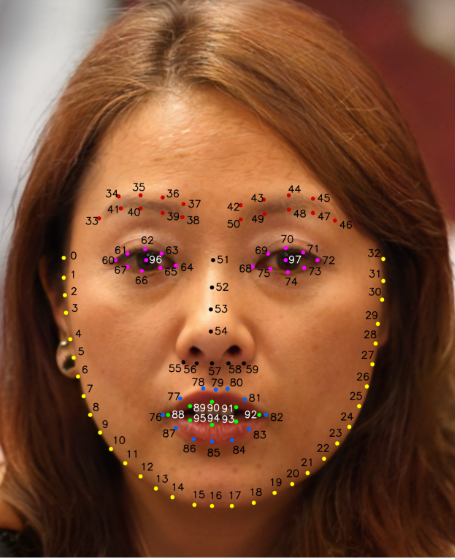
\includegraphics[width=.6\linewidth]{figures/landmark-face.png}
    \caption{Immagine dei landmark estratti dalla rete ADNet}
    \label{fig:landmark-face}
\end{figure}
\begin{itemize}
    \item dal 60 al 67: contorno occhio sinistro
    \item dal 68 al 75: contorno occhio destro
    \item 96: pupilla occhio sinistro
    \item 97: pupilla occhio destro
\end{itemize}

\section{Implementazione della metrica}
\subsection{Descrizione dell'algoritmo}
Viene inizialmente effettuata la segmentazione dell'occhio, l'algoritmo inizia isolando l'area dell'occhio dall'immagine completa utilizzando i landmarks forniti.
Una volta estratta la regione dell'occhio, l'algoritmo crea una maschera specifica per l'iride, escludendo sia la pupilla centrale (che appare normalmente scura) sia le aree esterne all'occhio. Questa segmentazione geometrica si basa su proporzioni anatomiche standard.
Lo scopo dell'algoritmo è ora quello di rilevare le zone dell'iride dove sono presenti pixel rosse, per eseguire questo compito è necessario convertire l'immagine dal tradizionale spazio colori RGB ad alcuni più utili all'isolamento di determinati colori all'interno dell'immagine quali : \begin{itemize}
    \item HSV: separa il colore dalla luminosità rendendo la misurazione meno sensibilile alle variazioni di luce
    \item yCbCr: separa luminanza da crominanza garantendo una misurazione più robusta a luce ed combre, inoltre, come illustrato dal paper "Face Detection in Color Images", questo spazio colore è ottimo per segmentare elementi facciali contraddistinti dal colore rosso.
\end{itemize}
Nel caso dello spazio colori HSV viene scelta una soglia di identificazione del colore rosso su tutti e tre i calanli.
Nel caso dello spazio colori yCbCr viene scelta una soglia minima per il canale cr, una massima per il canale cb ed inoltre vengono selezionati solamente i pixel con un valore di cr superiore alla medie per evitare problemi di saturazione.
In entrambi i casi le soglie sono state scelte in maniera sperimentale, cercando di rispettare un giosto connubio tra falsi positivi e falsi negativi.
Infine l'algoritmo calcola il rapporto tra i pixel rossi rilevati nell'iride e l'area totale dell'iride stessa, fornendo un valore normalizzato tra 0 e 1 che quantifica l'intensità dell'effetto occhi rossi.
La soglia di rosso è stata scelta in base ai risultati dei test, cercando di avere un giusto equilibrio tra falsi positivi e falsi negativi, come ad esempio le persone con gli occhi marrone o marrone chiaro.
\subsection{Dati di Input}
\begin{itemize}
    \item immagine: immagine digitale a colori
    \item puntiOcchio: vettore di punti che definiscono il contorno dell'occhio
    \item cornea: punto centrale della cornea
\end{itemize}
\subsection{Dati di Output}
\begin{itemize}
    \item rapportoRosso: valore decimale tra 0 e 1 che rappresenta la proporzione di pixel rossi nell'iride
\end{itemize}
\subsection{Algoritmo}
\begin{enumerate}
    \item Creazione maschera occhio [Fig. eye mask] \begin{itemize}
        \item Crea una maschera nera delle dimensioni dell'immagine
        \item Riempie l'area delimitata dai punti dell'occhio con bianco
        \item Calcola il rettangolo che racchiude l'occhio
    \end{itemize}
    \item Estrazione regione di interesse (ROI) \begin{itemize}
        \item Estrae la porzione di immagine corrispondente al rettangolo dell'occhio [Fig. eye roi]
        \item Estrae anche la corrispondente porzione di maschera dell'occhio [Fig. eye mask roi]
    \end{itemize}
    \item Calcolo parametri geometrici \begin{itemize}
        \item Calcola raggio pupilla = max(2, min(larghezza, altezza) / 8)
        \item Calcola raggio iride = altezza / 2
        \item Calcola centro pupilla rispetto alla ROI
    \end{itemize}
    \item Creazione maschera iride [Fig. iris mask] \begin{itemize}
        \item Crea maschera nera delle dimensioni della ROI
        \item Disegna cerchio bianco con raggio iride centrato sulla pupilla
        \item Disegna cerchio nero con raggio pupilla per escludere la pupilla centrale (la versione HSV è stata valutata sia con che senza questo passaggio)
    \end{itemize}
    \item Combinazione maschere [Fig. combined mask] \begin{itemize}
        \item Combina maschera occhio e maschera iride con operazione AND
        \item Risultato: maschera che isola solo la regione dell'iride
    \end{itemize}
    \item Rilevamento colore rosso [Fig. red mask] 
    \begin{itemize}
        \item Versione con HSV
            \begin{itemize}
                \item Converte l'immagine dell'occhio da BGR a HSV per migliore rilevamento colori
                \item Definisce soglie HSV per il colore rosso: \begin{itemize}
                    \item Gamma 1: H(0-10), S(100-255), V(50-255)
                    \item Gamma 2: H(160-180), S(100-255), V(50-255)
                \end{itemize}
                \item Crea maschere separate per ciascuna gamma
                \item Combina le maschere rosse con operazione OR
            \end{itemize}
        \item Versione con yCbCr
            \begin{itemize}
                \item Converte l'immagine dell'occhio da BGR a yCbCr
                \item Separa i canali cb e cr
                \item calcola media cr = la media dei valori della matrice cr
                \item calcola la matrice valoriAltiCr = maschera sui valori di cr maggiori di 150
                \item calcola la matrice valoriBassiCb = maschera sui valori di cb minori di 120
                \item calcola la matrice valoriMaggioreMediaCr = maschera sui valori di cr maggiori alla media cr
                \item calcola red mask = end logico bit a bit tra valoriAltiCr, valoriBassiCb, valoriMaggioreMediaCr
            \end{itemize}
    \end{itemize}
    \item Isolamento pixel rossi nell'iride [Fig. red iris mask] \begin{itemize}
        \item Applica maschera rossa alla maschera iride combinata
        \item Risultato: pixel rossi presenti solo nell'area dell'iride
    \end{itemize}
    \item Calcolo rapporto finale \begin{itemize}
        \item Conta pixel rossi nell'iride
        \item Conta pixel totali nell'area iride
        \item Se area iride $<$ 0: rapportoRosso = pixelRossi / pixelTotaliIride
        \item Altrimenti: rapportoRosso = 0
    \end{itemize}
    \item Ritorna rapportoRosso
\end{enumerate}
\begin{figure}
    \centering
    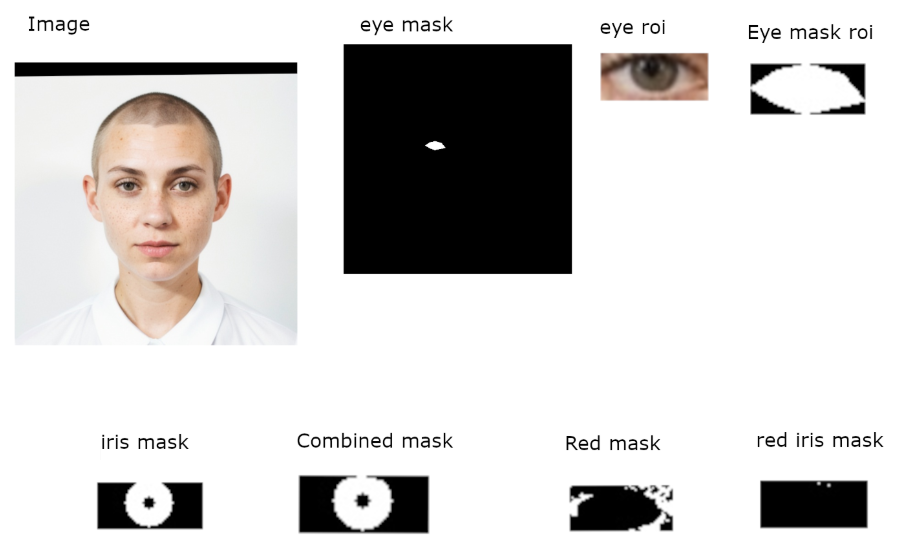
\includegraphics[width=1\linewidth]{figures/red-eye-process.png}
    \caption{Immagine descrittiva del procedimento per il rilevamento del difetto degli occhi rossi}
    \label{fig:red-eye-process}
\end{figure}

\chapter{Implementazione della metrica per il rilevamento dello sguardo frontale}

\section{Obbiettivo della metrica}
L’obiettivo della metrica è quello di assegnare uno score da 0 a 100 sul grado in cui un soggetto guarda in camera misura necessaria per garantire l’idoneità delle foto nei documenti di identità. Guardare dritto in camera è un requisito fondamentale per il riconoscimento facciale e per la conformità agli standard internazionali. 

\section{Requisiti preliminari}
I requisiti preliminari di questo task sono i landmark del viso. Il draft della ISO utilizza come riferimento per l'estrazione dei landmark facciali la CNN \href{https://github.com/huangyangyu/ADNet}{ADNet} allenata sul Wild dataset, prende in input un'immagine RGB e restituisce in output un set di 98 landmark \cref{fig:landmark-face}. I landmark che interessano questa metrica sono i seguenti:
\begin{itemize}
    \item 60, 64: angoli occhio sinistro
    \item 68, 72: angoli occhio destro
    \item 96: pupilla occhio sinistro
    \item 97: pupilla occhio destro
\end{itemize}

\section{Implementazione della metrica}


\subsection{Descrizione dell'algoritmo}
L'algoritmo analizza la direzione dello sguardo misurando la posizione delle pupille all'interno degli occhi. Per ogni occhio, calcola la larghezza totale (distanza tra gli angoli interno ed esterno) e la distanza tra la pupilla e l'angolo interno. Dividendo queste due misure ottiene un rapporto che indica dove si trova la pupilla: un valore di 0.5 significa che la pupilla è perfettamente centrata, mentre valori minori o maggiori indicano sguardo verso sinistra o destra. L'algoritmo confronta entrambi gli occhi e sceglie quello con maggiore deviazione dal centro per determinare la direzione principale dello sguardo. Infine, applica una trasformazione parabolica (con parametri alpha = -400 e beta = 100) che mappa il risultato su una scala da 0 a 100, dove valori più alti indicano maggiore deviazione dalla posizione frontale. Questo approccio permette di quantificare oggettivamente quanto una persona stia guardando lateralmente rispetto alla fotocamera.
Una visione grafica dei rapporti sopra elencati è disponibile 

\begin{figure}
    \centering
    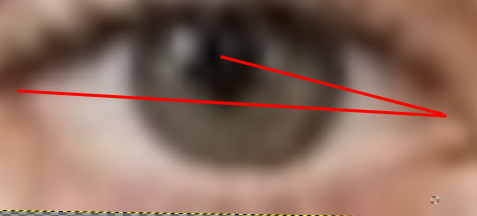
\includegraphics[width=.4\linewidth]{figures/frontal_gaze_manual.png}
    \caption{Immagine rappresentativa dei rapporti utilizzato dall'algoritmo di stima dello sguardo frontale manuale}
    \label{fig:frontal-gaze-manual}
\end{figure}

\subsection{Dati di Input}
\begin{itemize}
    \item a: coordinate x ed y dell'angolo esterno dell'occhio sinistro
    \item b: coordinate x ed y dell'angolo interno dell'occhio sinistro
    \item c: coordinate x ed y dell'angolo esterno dell'occhio destro
    \item d: coordinate x ed y dell'angolo interno dell'occhio destro
    \item e: coordinate x ed y della pupilla dell'occhio sinistro
    \item f: coordinate x ed y della pupilla dell'occhio destro
\end{itemize}
\subsection{Dati di Output}
\begin{itemize}
    \item valoreScalare: valore numerico che rappresenta la deviazione dello sguardo da 0 a 100
\end{itemize}
\subsection{Algoritmo}
\begin{enumerate}
    \item Calcolo larghezza degli occhi \begin{itemize}
        \item \(larghezzaSinistra = \sqrt{(b_x - a_x)^2 + (b_y - a_y)^2}\)
        \item \(larghezzaDestra = \sqrt{(d_x - c_x)^2 + (d_y - c_y)^2}\)
    \end{itemize}
    \item Calcolo distanza pupilla-angolo interno \begin{itemize}
        \item \(distanzaSinistra = \sqrt{(e_x - b_x)^2 + (e_y - b_y)^2}\)
        \item \(distanzaDestra = \sqrt{(f_x - d_x)^2 + (f_y - d_y)^2}\)
    \end{itemize}
    \item Calcolo rapporti normalizzati \begin{itemize}
        \item \(rapportoSinistro = \frac{distanzaSinistra}{larghezzaSinistra}\)
        \item \(rapportoDestro = \frac{distanzaDestra}{larghezzaDestra}\)
    \end{itemize}
    \item Calcolo variazioni dal centro (\textit{Nota: 0.5 rappresenta la posizione centrale ideale della pupilla}) \begin{itemize}
        \item \(variazioneSinistra = |rapportoSinistro - 0.5| \)
        \item \(variazioneDestra = |rapportoDestro - 0.5| \)
    \end{itemize}
    \item Selezione rapporto dominante \begin{itemize}
        \item Se \(variazioneDestra > variazioneDestra \) allora: \(punteggioGrezzo = rapportoSinistro \)
        \item Altrimenti: \(punteggioGrezzo = rapportoDestro\)
    \end{itemize}
    \item Applicazione funzione di scaling \begin{itemize}
        \item \(alpha = -400\)
        \item \(beta = 100 \)
        \item Calcola \(valoreScalare = alpha \cdot (punteggioGrezzo - \frac{1}{2})^2 + beta\)
    \end{itemize}
\end{enumerate}

\chapter{Rilevamento dello sguardo frontale tramite CNN}
\section{Selta del modello}
Dopo un'attenta analisi sui modelli stato dell'arte nel task del rilevamento dello sguardo si è trovato come riferimento l'implementazione della rete neurale descritta all'interno del paper \cite[L2CS-NET: FINE-GRAINED GAZE ESTIMATION IN UNCONSTRAINED ENVIRONMENTS]{10372944}.
Il modello descritto in questo paper si propone di prevedere lo sguardo in ambienti non vincolati, dando una stima degli angoli Pitch e Yaw del volto in radianti.

\section{Utilizzo del modello}
Il modello L2CS-NET viene distribuito sotto forma di pacchetto Python.
Il pacchetto espone un API tramite la quale è possibile far processare un'immagine ed ottenere per ogni volto dell'immagine gli angoli Pitch e Yaw.
Il modello L2CS-NET è costruito mediante il framework Pytorch ed è quindi un modello Pytorch, per poter utilizzare il modello all'interno del software OFIQ è necessario covnertire il modello al formato Onnx, un formato open utilizzato per rappresentare i modelli di machine learning.
Il formato Onnx permettere di eseguire il modello all'interno del software OFIQ in C++ tramite la libreria OnnxRuntime disponibile in C++.
Inoltre il pacchetto Python di L2CS-NET esegue il preprocessa dell'immagine tramite una pipeline che effettua i sueguenti step: \begin{itemize}
    \item Utilizza il modello RetinaFace (dalla libreria face detection) per trovare il bounding box dei vari volti all'interno dell'immagine
    \item Per ogni volto viene presa in considerazione solamente la parte dell'immagine compresa all'interno della bounding box (regione di interesse)
    \item Per ogni regione di interesse viene convertito lo spazio colori da BGR a RGB
    \item Ogni regione di interesse viene ridimensionato in un'immagine (224 * 224)
    \item Ogni regione di interesse viene passata al modello ResNet-50 seguito da 2 layer fully-connected che ritornano in output 90 classi rappresentanti intervalli discreti (sia per pitch che per yaw) con all'interno un valore rappresentante la probabilità che lo sguardo per il relativo angolo si trovi in quell'intervallo
    \item Per ogni valore ritornato da ResNet-50 viene applicata la funzione Softmax di modo da avere la probabilità in percentuale che lo sguardo si trovi all'interno di quell'intervallo
    \item Vengono moltiplicate le probabilità che lo sguardo si trovi in quell'intervallo per l'indice della probabilità nel vettore dei tensori
    \item Viene fatta la somma dei valori ottenuti precedentemente
    \item La somma viene moltiplicata per quattro ed il risultato sottratto di 180, in modo da convertire ogni probabilità ottenuta gradi.
    \item Viene eseguita la conversione da gradi a radianti
\end{itemize}
I passaggi che includono l'utilizzo di open cv sono facilmente replicabili all'interno del software OFIQ tramite la libreria open cv per cpp, mentre per trovare il bounding box del volto all'interno dell'immagine viene utilizzato il modello "SSD Face Detector CNN" che riporta risultati molto simili a quelli di RetinaFace, la scelta di utilizzare questo modello è dettata dal fatto di averlo già a disposizione all'interno del software in formato Onnx.

\section{Implementazione della metrica}

\subsection{Dati di Input}
\begin{itemize}
    \item immagine: L'immagine del volto da valutare
\end{itemize}
\subsection{Dati di Output}
\begin{itemize}
    \item valoreScalare: valore numerico che rappresenta la deviazione dello sguardo da 0 a 100
\end{itemize}
\subsection{Algoritmo}
\begin{enumerate}
    \item Calcola \(detectedFaces\) tramite il modello SSD Face Detector CNN
    \item Se \(detectedFaces.length < 1\) allora: \(valoreScalare = 0\). Fine.
    \item \(faceBoundingBox = detectedFaces[0]\), solamente il primo volto trovato verrà valutato
    \item Carica il modello in formato onnx tramite onnxRuntime
    \item Calcola \(immagineVolto\) = la sezione di immagine all'interno di \(faceBoundingBox\)
    \item Preprocessing per L2CS-NET \begin{itemize}
        \item Definisce \(inputSize = 443\)
        \item Calcola \(immagineRidimensionata\) ridimensionando con open cv \(immagineVolto\) alla grandezza (\(inputSize\) x \(inputSize\))
        \item Converte lo schema colore di \(immagineRidimensionata\) da BGR a RGB
        \item Scala i valori dell'immagine dall'intervallo [0,255] a [0,1] convertendoli a float
        \item Normalizza l'immagine \begin{itemize}
            \item Definisce \(mean = [0.485f, 0.456f, 0.406f]\) (dal preprocessing della librerie L2CS-NET)
            \item Definisce \(std = [0.229f, 0.224f, 0.225f]\) (dal preprocessing della librerie L2CS-NET)
            \item Per ogni canale RGB dell'immagine: \(channels[i] = \frac{(channels[i] - mean[i])}{std[i]}\) con \(i = 0..3\)
            \item Definisce \(immaginePreprocessata\) la matrice formata dai canali normalizzati nei punti precedenti
        \end{itemize}
        \item Definisce \(input_shape = [1, 3, inputSize, inputSize]\) (aggiunge la dimensione della batch (in questo caso 1 dato che viene processata solamente un'immagine))
        \item Converte l'input in una matrice CHW: \begin{itemize}
            \item Per ogni canale \(c = 0..3\): 
            \item Per ogni riga dell'immagine \(h = 0...inputSize\) 
            \item Per ogni colonna dell'immagine \(w = 0...inputSize\) 
            \item \(tensoreInput[c * inputSize * inputSize + h * inputSize + w] = immaginePreprocessata[h][w][c]\)
        \end{itemize}
    \end{itemize}
    \item Vengono usate le API offerte da \(onnxRuntime\) per eseguire il modello L2CS in formato Onnx. 
    \item Vengono calcolati \(pitch\) e \(yaw\) sulla base dell'output del modello (il modello restituisce in output i valori per 90 classi sia per pitch che per yaw, i seguenti step vengono eseguiti per entrambi gli angoli) 
    \item \begin{itemize} 
        \item Sia \(x\) il vettore con i 90 valori
        \item \(angoloInRadianti = \frac{\sum_{i}^{x} (e^{x_i}*i)}{\sum_i^{x}(e^x)}\) * 4 - 180
    \end{itemize}
    \item \( value = max(|pitch|, |yaw|) \) (Si usa il valore assoluto in quanto lo sguardo frontale viene classificato come angolo 0)
    \item \( score = round((1 - (\frac{min(value, 45)}{45}))*100) \) (Uso 45 come valore limite, tutti valore da 45 a 180 vengono classificati come punteggio 0)
    \item value è il valore assoluto dell'angolo più lontano da 0 Gradi, mentre score è la valutazione dell'immagine da 0 a 100
\end{enumerate}

\chapter{Rilevamento dello sguardo frontale tramite Machine Learning}
\label{chap:frontal_gaze_with_ml}

L'utilizzo di metodi algoritmici basati sulle coordinate dei landmark, insieme a modelli in grado di predire l'angolazione dello sguardo, rappresenta un approccio valido per determinare se un volto stia guardando in fotocamera. Esistono tuttavia ulteriori strategie degne di nota. Questo capitolo è dedicato a tre approcci alternativi sviluppati per stabilire se uno sguardo sia rivolto verso la camera.

\section{Fine-Tuning di modelli CNN}
\label{chap:mobilenetv2_ft}

In questa sezione viene approfondito l'utilizzo di reti neurali convoluzionali preaddestrate come classificatori, successivamente adattate tramite la tecnica del \textit{Fine-Tuning}, con l'obiettivo di predire se un volto presenti lo sguardo diretto in camera.  

Per eseguire i test è stato necessario disporre di un dataset di grandi dimensioni con dati reali. La scelta è ricaduta sul dataset \href{https://www.kaggle.com/datasets/estopadilla/gaze-direction-detection}{Gaze Direction Detection}, disponibile sulla piattaforma Kaggle.  

Il dataset contiene circa 53000 coppie di occhi ed è rilasciato sotto forma di array binario \texttt{numpy} (.npz), al cui interno sono presenti tre array principali:
\begin{itemize}
    \item \texttt{targets}: contiene valori binari (0 e 1), dove l'elemento $i$-esimo indica se lo sguardo corrispondente negli altri array è rivolto in camera (1) oppure altrove (0).
    \item \texttt{right\_eyes}: immagini raffiguranti gli occhi destri.
    \item \texttt{left\_eyes}: immagini raffiguranti gli occhi sinistri.
\end{itemize}

Ogni immagine ha dimensioni \(64 \times 64\) e raffigura un occhio con una piccola porzione del volto, comprendendo, a volte, anche parte del naso.  
Il dataset è stato suddiviso in training set (40000 immagini) e test set (4000 immagini), bilanciati in termini di immagini con sguardo in camera e non.  

Il Fine-Tuning è stato eseguito sul modello MobileNetV2, la cui architettura è descritta in \cite{Sandler2018MobileNetV2IR}. Il layer di output è stato sostituito con un layer denso (\texttt{Dense}) di 2 nodi con funzione di attivazione \texttt{softmax}. L'addestramento è stato condotto con l’ottimizzatore \texttt{Adam} e come funzione di loss \texttt{categorical\_crossentropy}.  

Sono inoltre stati adottati i seguenti accorgimenti:
\begin{itemize}
    \item \textbf{Early stopping}: interruzione dell'addestramento se, per $n$ epoche consecutive, non si osservano miglioramenti della loss, mantenendo i pesi relativi al miglior risultato.
    \item Addestramento iniziale dei soli strati finali, mantenendo congelati gli altri.
    \item Successivo addestramento dell'intera rete.
\end{itemize}

\subsection{Fine-Tuning di MobileNetV2 - versione 1}
\label{chap:mobilenetv2_ft_v1}

Nella prima versione il modello è stato addestrato direttamente sulle immagini originali del dataset ``Gaze Direction Detection''.  

\textbf{Accuracy sul test set}: 74.0\%.  

La matrice di confusione è riportata in \Cref{fig:fine_tuning_mobilenetv2_version_1_confusion_matrix}.  

Per integrare il modello in OFIQ,  è stato esportato in formato ONNX e affiancato da una pipeline di preprocessing delle immagini, così strutturata:
\begin{itemize}
    \item Costruzione di un bounding box attorno ai landmark dell'occhio rilevati da ADNet.
    \item Individuazione del lato maggiore del bounding box e moltiplicazione per un fattore di scala (2.5).
    \item Ricostruzione del bounding box mantenendo l'occhio al centro.
    \item Ridimensionamento dell'immagine a \(224 \times 224\), dimensione richiesta da MobileNetV2.
    \item Inferenza tramite il modello, che restituisce due valori: probabilità di sguardo frontale (tensore 0) e probabilità contraria (tensore 1).
\end{itemize}

\begin{figure}
    \centering
    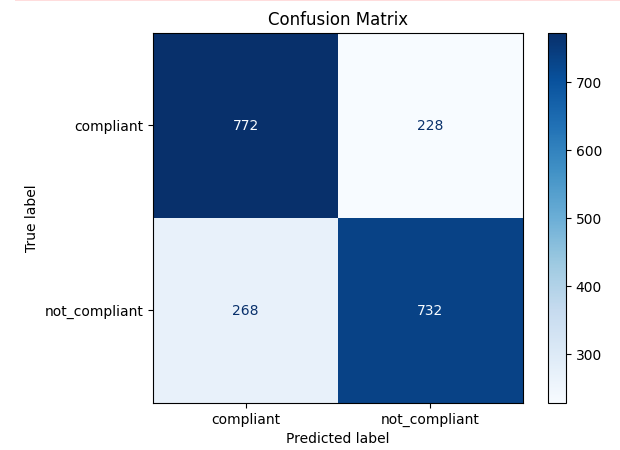
\includegraphics[width=.6\linewidth]{figures/fine-tuning-mobilenetv2-version-1-confusion-matrix.png}
    \caption{Matrice di confusione del Fine-Tuning di MobileNetV2, versione 1}
    \label{fig:fine_tuning_mobilenetv2_version_1_confusion_matrix}
\end{figure}

\subsection{Fine-Tuning di MobileNetV2 - versione 2}
\label{chap:mobilenetv2_ft_v2}

Poiché la versione 1 mostrava buoni risultati sul test set ma scarsa capacità di generalizzazione su dataset differenti, nella versione 2 si è intervenuti sul preprocessing, facendo in modo che il modello valutasse esclusivamente l'occhio.  

Il preprocessing adottato è il seguente:
\begin{itemize}
    \item Rilevamento degli occhi tramite classificatore HaarCascade di OpenCV.
    \item Ritaglio del bounding box dell'occhio.
    \item Ridimensionamento a \(96 \times 96\).
    \item Aggiunta di un bordo nero fino a raggiungere \(224 \times 224\), così da preservare le proporzioni senza introdurre rumore eccessivo.
\end{itemize}

\textbf{Accuracy sul test set}: 78.4\%.  

La matrice di confusione è riportata in \Cref{fig:fine_tuning_mobilenetv2_version_2_confusion_matrix}.  

\begin{figure}
    \centering
    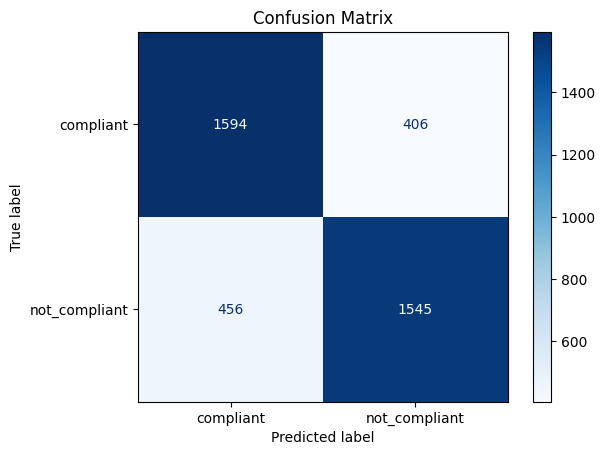
\includegraphics[width=.6\linewidth]{figures/fine-tuning-mobilenetv2-version-2-confusion-matrix.png}
    \caption{Matrice di confusione del Fine-Tuning di MobileNetV2, versione 2}
    \label{fig:fine_tuning_mobilenetv2_version_2_confusion_matrix}
\end{figure}

\section{Costruzione di un modello CNN \texttt{gdd CNN}}
\label{chap:build_cnn_model}

Per ridurre l'impatto del rumore dovuto al ridimensionamento e a particolari tecniche di preprocessing, è stato implementato un modello CNN da zero, accettando in input immagini di dimensione \(96 \times 96\).  

La struttura del modello, illustrata in \Cref{fig:custom_CNN_architecture}, comprende 4 blocchi alternati di convoluzione e max pooling, fino a ottenere una dimensione di \(6 \times 6 \times 256\). Segue una rete fully connected con 512 nodi, un layer di dropout e infine il layer di output con 2 classi e funzione di attivazione \texttt{softmax}.  

Addestramento:
\begin{itemize}
    \item Ottimizzatore: \texttt{Adam}.
    \item Funzione di loss: \texttt{sparse\_categorical\_crossentropy}.
    \item Early stopping.
\end{itemize}

Il modello è stato addestrato sul dataset ``Gaze Direction Detection'' e successivamente convertito in formato ONNX per l'integrazione in OFIQ.  

Pipeline di preprocessing:
\begin{itemize}
    \item Rilevamento dell'occhio con HaarCascade di OpenCV.
    \item Ritaglio del bounding box dell'occhio;
    \item Ridimensionamento a \(96 \times 96\).
\end{itemize}

\textbf{Accuracy sul test set}: 85.0\%.  

La matrice di confusione è riportata in \Cref{fig:custom_cnn_confusion_matrix}.  

Il modello è stato denominato \texttt{gdd CNN} (\texttt{Gaze Direction Detector CNN}).

\begin{figure}
    \centering
    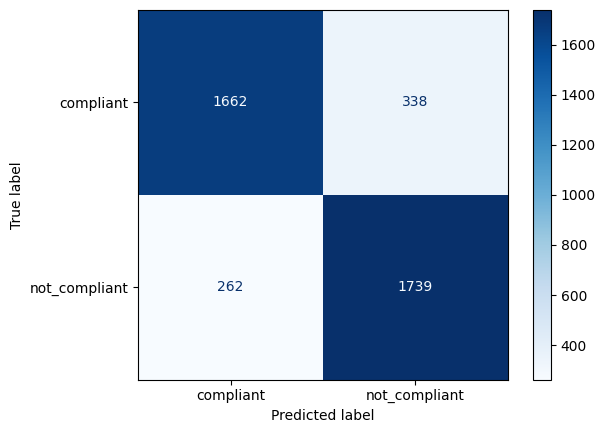
\includegraphics[width=.6\linewidth]{figures/custom-cnn-confusion-matrix.png}
    \caption{Matrice di confusione del modello CNN sviluppato da zero}
    \label{fig:custom_cnn_confusion_matrix}
\end{figure}

\begin{figure}
    \centering
    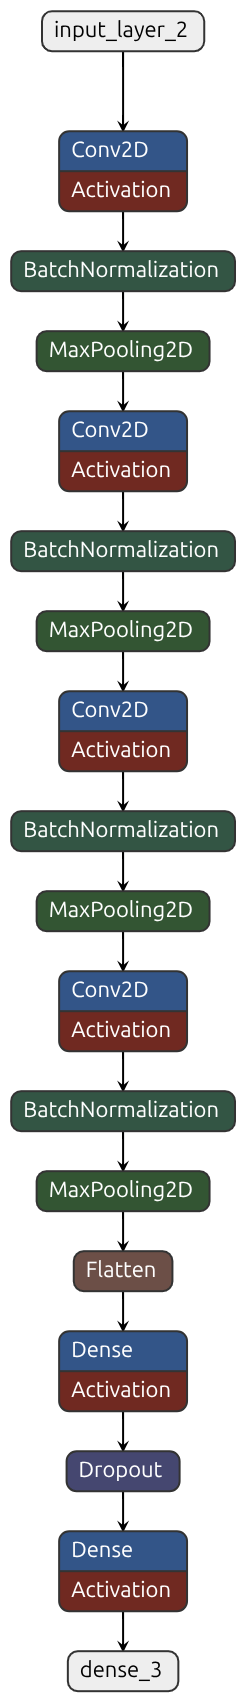
\includegraphics[width=.2\linewidth]{figures/custom-CNN-architecture}
    \caption{Architettura della CNN implementata}
    \label{fig:custom_CNN_architecture}
\end{figure}

\section{Modelli di machine learning basati sui landmark facciali}
\label{chap:landmark_based_model}

Per affrontare i problemi di generalizzazione emersi nei modelli CNN, è stata sviluppata una soluzione basata sull'estrazione dei landmark facciali e sul loro utilizzo come input per modelli di machine learning.  

Struttura generale:
\begin{itemize}
    \item \textbf{Estrattore di landmark}: due approcci testati
    \begin{itemize}
        \item \textbf{MediaPipe Face Mesh} (20 landmark per occhio, comprensivi dell'iride, Paper~\cite{48292}).
        \item \textbf{ADNet} (9 landmark per occhio).
    \end{itemize}
    \item \textbf{DataFrame pandas}: per la gestione dei landmark.
    \item \textbf{Modello predittivo}: 
    \begin{itemize}
        \item \textbf{XGBoost}.
        \item Rete neurale fully connected in Keras (input layer con un neurone per colonna, hidden layer da 128 neuroni, output layer con un neurone e attivazione \texttt{sigmoid}).
    \end{itemize}
\end{itemize}

L'addestramento ha utilizzato la tecnica della \textit{K-Fold Cross Validation}, con landmark normalizzati per favorire la generalizzazione.  

Dataset:
\begin{itemize}
    \item \textbf{ONOT}: immagini con sguardo in camera;
    \item \textbf{TONO}: immagini con sguardo non in camera;
\end{itemize}
per un totale di circa 1.000 immagini.  

Il dataset ``Gaze Direction Detection'' non è stato utilizzato poiché non includeva il volto completo, necessario agli estrattori di landmark. I modelli sono stati inoltre testati su un sotto-dataset di immagini reali fornite da Biolab, tutte con sguardo frontale.

\subsection{Risultati dei modelli basati su landmark}

\begin{itemize}
    \item \textbf{MediaPipe Face Mesh + XGBoost}  
    Accuracy: 77.0\%,  Equal Error Rate: 26.5\%,  Accuracy Biolab: 63.2\%.  
    Matrice di confusione: \Cref{fig:mediapipe_xgboost_confusion_matrix}.
    
    \item \textbf{MediaPipe Face Mesh + Keras}  
    Accuracy: 64.0\%,  Equal Error Rate: 50.0\%,  Accuracy Biolab: 0.0\%.  
    Matrice di confusione: \Cref{fig:mediapipe_keras_confusion_matrix}.
    
    \item \textbf{ADNet + XGBoost}  
    Accuracy: 64.3\%,  Equal Error Rate: 43.1\%,  Accuracy Biolab: 12.1\%.  
    Matrice di confusione: \Cref{fig:adnet_xgboost_confusion_matrix}.
    
    \item \textbf{ADNet + Keras}  
    Accuracy: 69.5\%,  Equal Error Rate: 50.0\%,  Accuracy Biolab: 0.0\%.  
    Matrice di confusione: \Cref{fig:adnet_keras_confusion_matrix}.
\end{itemize}

\begin{figure}[htbp]
    \centering
    \begin{subfigure}{0.45\textwidth}
        \centering
        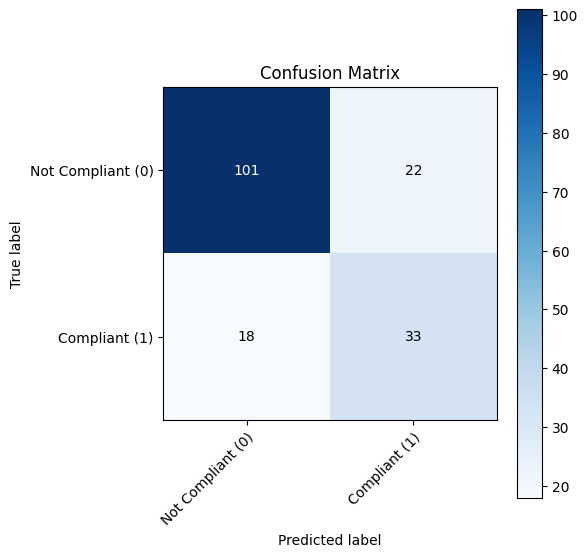
\includegraphics[width=\linewidth]{figures/mediapipe_xgboost_confusion_matrix.png}
        \caption{MediaPipe + XGBoost}
        \label{fig:mediapipe_xgboost_confusion_matrix}
    \end{subfigure}
    \hfill
    \begin{subfigure}{0.45\textwidth}
        \centering
        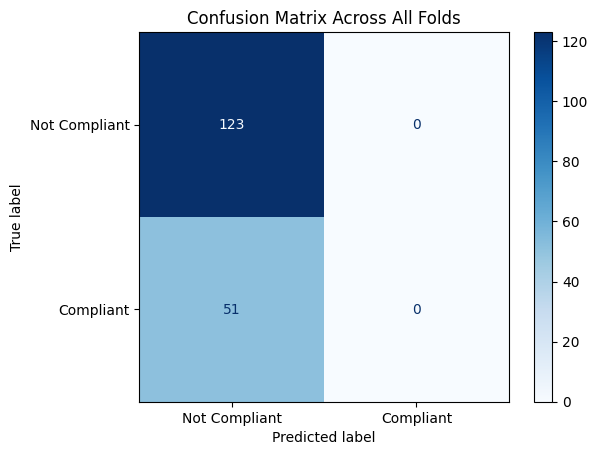
\includegraphics[width=\linewidth]{figures/mediapipe_keras_confusion_matrix.png}
        \caption{MediaPipe + Keras}
        \label{fig:mediapipe_keras_confusion_matrix}
    \end{subfigure}
    \begin{subfigure}{0.45\textwidth}
        \centering
        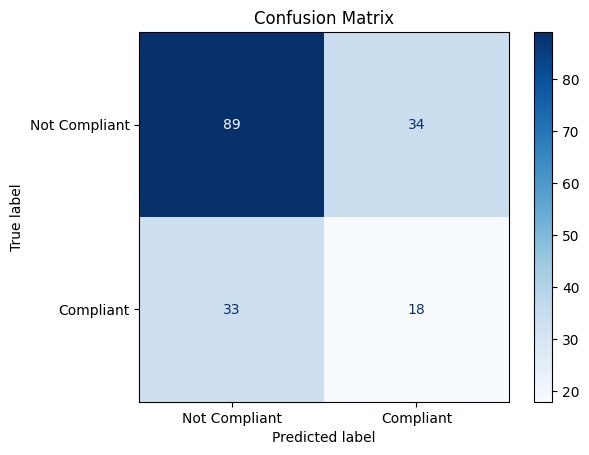
\includegraphics[width=\linewidth]{figures/adnet_xgboost_confusion_matrix.png}
        \caption{ADNet + XGBoost}
        \label{fig:adnet_xgboost_confusion_matrix}
    \end{subfigure}
    \hfill
    \begin{subfigure}{0.45\textwidth}
        \centering
        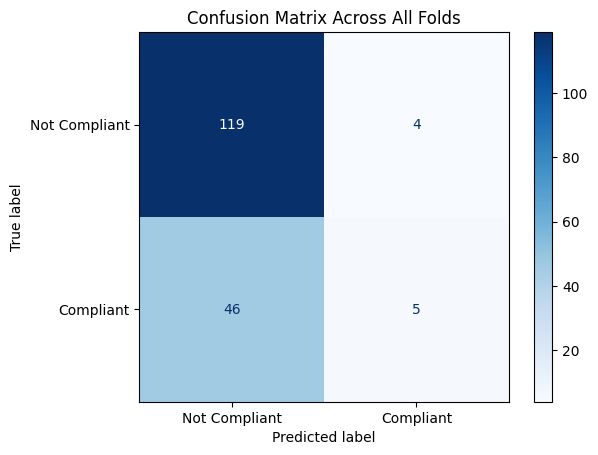
\includegraphics[width=\linewidth]{figures/adnet_keras_confusion_matrix.png}
        \caption{ADNet + Keras}
        \label{fig:adnet_keras_confusion_matrix}
    \end{subfigure}
    \caption{Matrici di confusione dei modelli basati su landmark facciali}
\end{figure}



\chapter{Strumenti utilizzati per lo sviluppo delle metriche}

\section{Software OFIQ}
Il software OFIQ, acronimo di \textit{Open Source Face Image Quality}, è un progetto open source sviluppato per implementare le metriche descritte nel draft dello standard ISO 29794-5.
È scritto in linguaggio C++ e dispone di file CMake per la compilazione su sistemi Linux, Windows e macOS.
Al suo interno utilizza librerie come OpenCV per la gestione delle immagini e OnnxRuntime per l'esecuzione dei modelli Onnx.
Inizialmente presentava un'implementazione fedele di tutte le metriche riportate nello standard ISO 29794-5, restituendo in output un valore grezzo ed un valore normalizzato tra 0 e 100 (utile come \textit{score}) per ciascuna metrica.
OFIQ include inoltre delle utility che permettono l'utilizzo dei seguenti modelli (in formato Onnx): 
\begin{itemize}
    \item SSD Face Detector CNN: modello per il rilevamento dei volti in un'immagine.
    \item ADNet: modello per l'estrazione dei landmark facciali.
\end{itemize}

Il software implementa le seguenti metriche: 
\begin{itemize}
    \item Quality Score: uno score generale dell'immagine ottenuto tramite il modello MagFace.
    \item Background uniformity: misura l'uniformità dello sfondo.
    \item Illumination uniformity: misura l'uniformità dell'illuminazione confrontando la parte destra e sinistra del volto.
    \item Luminance mean: verifica che l'immagine presenti un'illuminazione adeguata e uniforme.
    \item Luminance variance: misura i contrasti nell'immagine.
    \item Under-exposure prevention: verifica che l'immagine non contenga troppi pixel con bassa luminosità.
    \item Over-exposure prevention: verifica che l'immagine non contenga troppi pixel con alta luminosità.
    \item Dynamic range: misura la variazione di intensità luminosa nella regione del volto, assicurando che non sia completamente scura o chiara.
    \item Sharpness: valuta la nitidezza dell'immagine (corretta messa a fuoco).
    \item No compression artifacts: valuta la presenza di artefatti di compressione, assicurando che l'immagine non sia stata eccessivamente compressa.
    \item Natural colour: valuta la naturalezza del colore della pelle.
    \item Single face present: verifica la presenza di un singolo volto.
    \item Eyes open: controlla che entrambi gli occhi siano aperti in modo naturale.
    \item Mouth closed: verifica che la bocca sia chiusa.
    \item Eyes visible: verifica che siano visibili pupilla e iride in entrambi gli occhi.
    \item Mouth occlusion prevention: controlla che la bocca non sia occlusa.
    \item Face occlusion prevention: verifica che la regione del volto (dalla sommità del capo al mento e da orecchio a orecchio) sia chiaramente visibile.
    \item Inter-eye distance: misura in pixel la distanza tra gli occhi.
    \item Head size: valuta la dimensione del volto per evitare immagini troppo ravvicinate.
    \item Leftward crop of face: verifica che il volto non sia decentrato a sinistra.
    \item Rightward crop of face: verifica che il volto non sia decentrato a destra.
    \item Downward crop of face: verifica che il volto non sia decentrato in basso.
    \item Upward crop of face: verifica che il volto non sia decentrato in alto.
    \item Pose angle yaw frontal alignment: verifica che l'angolo \textit{yaw} del volto sia inferiore a \(\pm 5^\circ\) dal frontale.
    \item Pose angle pitch frontal alignment: verifica che l'angolo \textit{pitch} del volto sia inferiore a \(\pm 5^\circ\) dal frontale.
    \item Pose angle roll frontal alignment: verifica che l'angolo \textit{roll} del volto sia inferiore a \(\pm 8^\circ\) dal frontale.
    \item Expression neutrality: verifica che il volto presenti un'espressione neutrale.
    \item No head covering: verifica che il soggetto non indossi copricapi (ad esempio un cappello).
\end{itemize}

\section{Dataset utilizzati per la valutazione}
I seguenti dataset sono stati utilizzati per la valutazione delle metriche implementate.

\subsection{ONOT}
ONOT è un dataset introdotto nel paper \cite[ONOT: a High-Quality ICAO-compliant Synthetic Mugshot Dataset]{di2024onot}.
È composto da immagini sintetiche di alta qualità conformi ai requisiti dello standard ISO/IEC 39794-5.
Quest'ultimo definisce un formato per lo scambio di immagini facciali negli \textit{electronic Machine-Readable Travel Documents} (eMRTD), seguendo le linee guida dell'International Civil Aviation Organization (ICAO).
Le immagini di ONOT includono volti di diverse etnie, età, generi e caratteristiche facciali, rendendo il dataset adatto alla valutazione delle metriche implementate.
Per questa analisi sono state considerate le sole immagini del \textit{Subset 1}, ICAO compliant.

\subsection{TONO}
TONO è un dataset introdotto nel paper \cite[TONO: a synthetic dataset for face image compliance to ISO/ICAO standard]{borghi2024tono}.
È costituito da immagini sintetiche di volti ad alta qualità, create per sviluppare e valutare sistemi di verifica della conformità delle immagini facciali allo standard ISO/ICAO.
Le immagini di TONO derivano dal dataset ONOT (\cite{di2024onot}), con l'aggiunta di uno o più elementi non conformi agli standard.
I difetti presenti in TONO sono i seguenti: 
\begin{itemize}
    \item Head and Shoulder Pose: assenza di posa frontale sia del volto che delle spalle.
    \item Gaze Direction: assenza di sguardo frontale.
    \item Expression: mancanza di espressione neutrale o presenza di denti visibili.
    \item Face Illumination: non uniformità dell'illuminazione del volto.
    \item Background: sfondo non uniforme.
    \item Head Coverings: presenza di copricapi.
    \item Eye Visibility: occhi chiusi, presenza di occhiali (da vista o da sole), make-up eccessivo.
    \item Photographic: difetti quali pixelazione, posterizzazione, sfocatura, sovraesposizione, sovrasaturazione.
\end{itemize}
Per questa casistica è stata utilizzata la versione di TONO in cui ogni immagine contiene un solo elemento in contrasto con i requisiti ISO/ICAO.

\section{Onnx e OnnxRuntime}
ONNX (\textit{Open Neural Network Exchange}) è un formato open source per la rappresentazione di modelli di machine learning, progettato per garantire compatibilità tra diversi framework (PyTorch, TensorFlow, ecc.).
Permette di salvare un modello in un file \texttt{.onnx} indipendente dall'ambiente di training.
La libreria OnnxRuntime fornisce API utilizzabili da diversi linguaggi di programmazione e su diverse piattaforme (inclusi i web browser).
Il progetto, sviluppato da Microsoft, è disponibile al seguente repository GitHub: \href{https://github.com/microsoft/onnxruntime}{https://github.com/microsoft/onnxruntime}.

\section{FVC Ongoing}
FVC Ongoing (\cite{fvcongoing}) è una piattaforma web che consente la valutazione di algoritmi di vario tipo, tra cui il task \textit{Face Image ISO Compliance Verification}.
I test vengono condotti su diversi dataset e metriche note.

\section{Framework PyTorch}
Il linguaggio di programmazione Python ed il framework PyTorch sono comunemente utilizzati per l'addestramento e la distribuzione di modelli di Machine Learning. 
Nel progetto il loro impiego riguarda principalmente il testing e la conversione in formato Onnx del modello L2CS-Net, originariamente distribuito in PyTorch.
In particolare, è stato utilizzato il modulo \texttt{ONNX exporter API}, che consente di esportare un modello PyTorch in formato Onnx, impiegato per la conversione di L2CS-Net tramite il seguente codice: \cref{lst:onnx-exporter}
\lstinputlisting[float,language=Python,label={lst:onnx-exporter}]{listings/onnx_exporter.py}

\section{Libreria Keras}
Keras è una libreria open-source di alto livello per il \textit{deep learning}, scritta in Python e basata sul motore di calcolo TensorFlow.  
Nel presente lavoro, Keras è stata utilizzata per:
\begin{itemize}
    \item Eseguire il Fine-Tuning di MobileNetV2 (Sezione~\ref{chap:mobilenetv2_ft}).
    \item Sviluppare la rete CNN descritta nella Sezione~\ref{chap:build_cnn_model}.
    \item Implementare la rete neurale fully connected basata sui landmark (Sezione~\ref{chap:landmark_based_model}).
\end{itemize}

\section{Libreria XGBoost}
La libreria \texttt{XGBoost} (\textit{eXtreme Gradient Boosting}) \cite{xgboost} mette a disposizione il modulo \texttt{XGBoostClassifier}, che consente di utilizzare modelli basati su alberi decisionali ottimizzati tramite l'algoritmo del Gradient Boosting per la risoluzione di problemi di classificazione.  
In questo lavoro, XGBoost è stato impiegato per costruire due dei modelli basati sui landmark (Sezione~\ref{chap:landmark_based_model}).


\section{Jupyter Notebook, Numpy e Matplotlib}
Jupyter Notebook, Numpy e Matplotlib sono stati utilizzati per creare documenti interattivi e rappresentare graficamente (tramite boxplot e istogrammi) le performance delle metriche di valutazione sui dataset ONOT, TONO e su un sottoinsieme di Biolab.
Il linguaggio Python è stato inoltre impiegato per:
\begin{itemize}
    \item suddividere i dataset in base ai file di riferimento in formato \texttt{.txt};
    \item elaborare le metriche per valutare il software OFIQ e gli algoritmi proposti.
\end{itemize}

\chapter{Valutazione delle metriche}

\section{Introduzione alle valutazioni}
Per quanto riguarda le valutazioni del software OFIQ, verranno riportati ed analizzati esclusivamente i risultati delle metriche implementate nelle loro diverse versioni. 
In particolare, per ogni metrica saranno presi in esame l'\texttt{Equal Error Rate} e la distribuzione dei risultati.

\section{Valutazione su FVC-Ongoing}

\subsection{Metriche valutate}
La piattaforma FVC-Ongoing valuta 24 diverse metriche \cref{tab:fvc-table}.
Nel caso di questo progetto, le metriche selezionate sono:
\begin{itemize}
    \item Looking Away: valuta se un soggetto sta guardando in camera.
    \item Red Eyes: valuta la presenza del difetto degli occhi rossi.
\end{itemize}

\begin{table}[h!]
\centering
\begin{tabular}{|c|p{10cm}|}
\hline
\textbf{N°} & \textbf{Description of the test} \\
\hline
\multicolumn{2}{|l|}{\textbf{Feature extraction accuracy tests}} \\
\hline
1 & Eye center location accuracy \\
\hline
\multicolumn{2}{|l|}{\textbf{Photographic and pose-specific tests}} \\
\hline
2 & Blurred \\
3 & Looking away \\
4 & Ink marked/creased \\
5 & Unnatural skin tone \\
6 & Too dark/light \\
7 & Washed out \\
8 & Pixelation \\
9 & Hair across eyes \\
10 & Eyes closed \\
11 & Varied background \\
12 & Roll/pitch/yaw $>$ predefined thresholds \\
13 & Flash reflection on skin \\
14 & Red eyes \\
15 & Shadows behind head \\
16 & Shadows across face \\
17 & Dark tinted lenses \\
18 & Flash reflection on lenses \\
19 & Frames too heavy \\
20 & Frame covering eyes \\
21 & Hat/cap \\
22 & Veil over face \\
23 & Mouth open \\
24 & Other faces/toys too close \\
\hline
\end{tabular}
\caption{Metriche valutate da FVC-Ongoing}
\label{tab:fvc-table}
\end{table}

\subsection{Il protocollo}
Per la sottomissione degli algoritmi sulla piattaforma FVC-Ongoing è necessario rispettare il seguente protocollo:
\begin{itemize}
    \item inviare una cartella compressa in formato ZIP;
    \item all'interno deve essere presente un file \textit{Check.exe}, eseguibile per Win32 in formato \textit{console application};
    \item la sintassi da riga di comando deve essere: \texttt{./Check.exe <faceimagefile> <outputfile>}, dove:
    \begin{itemize}
        \item \texttt{faceimagefile}: percorso dell'immagine del volto da valutare (formati supportati: BMP, JPG, PNG);
        \item \texttt{outputfile}: percorso del file TXT di output, su cui scrivere (in modalità \textit{append}) l'esito dei test.
    \end{itemize}
    \item Ogni riga del file di output deve contenere i seguenti campi separati da spazi:
    \begin{itemize}
        \item \texttt{ImageName}: nome del file immagine;
        \item \texttt{RetVal}: intero che indica se l'immagine può essere processata:
        \begin{itemize}
            \item 1: immagine processabile;
            \item 0: immagine non processabile;
            \item -1: dimensione dell'immagine non supportata;
            \item -2: formato immagine non supportato;
            \item -3: contenuto non processabile.
        \end{itemize}
        \item \texttt{LE\_x}, \texttt{LE\_y}: coordinate X e Y del centro dell'occhio sinistro (in pixel);
        \item \texttt{RE\_x}, \texttt{RE\_y}: coordinate X e Y del centro dell'occhio destro (in pixel);
        \item \texttt{Test\_2}: intero compreso tra 0 e 100 indicante il grado di conformità rispetto al test 2 (0 = non conforme, 100 = massimo livello di conformità). In alternativa, può assumere i valori:
        \begin{itemize}
            \item \texttt{-}: se la metrica non è supportata dal programma;
            \item \texttt{?}: se la metrica è supportata ma non valutabile nell'immagine corrente per un motivo specifico;
            \item \texttt{!}: se la metrica è supportata ma non valutabile nell'immagine corrente per motivo indefinito.
        \end{itemize}
        \item ...
        \item \texttt{Test\_24}: analogo al campo \texttt{Test\_2}, relativo al test 24.
    \end{itemize}
    \item L'eseguibile deve avere permessi di scrittura solo sul file di output, mentre i file di configurazione possono essere caricati esclusivamente in lettura.
\end{itemize}

Dopo un'attenta analisi del protocollo richiesto dalla piattaforma FVC-Ongoing, è stato necessario rendere il software OFIQ conforme a tali specifiche ed adattare le metriche implementate.

\subsection{Valutazione metrica per il rilevamento del difetto degli occhi rossi (versione HSV)}
La valutazione della metrica per il difetto degli occhi rossi è divisa in due parti. 
Nella prima parte vengono analizzati i risultati ottenuti tramite l'algoritmo basato sullo spazio colore HSV, mentre nella seconda parte si utilizza lo spazio colore yCbCr. \\[4pt]
\texttt{Equal Error Rate}: 18.1\%. \\
La distribuzione degli score è riportata nel grafico \Cref{fig:score_distribution_red_eye_with_hsv}. 

\begin{figure}
    \centering
    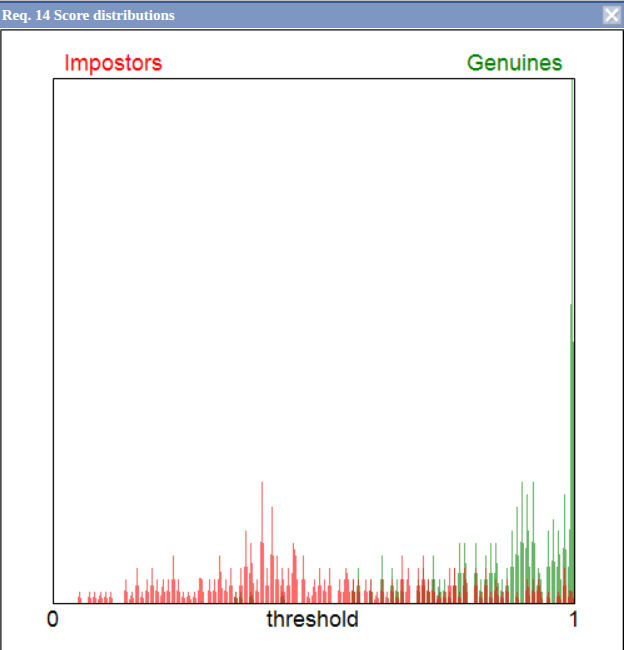
\includegraphics[width=.8\linewidth]{figures/score-distribution-red-eye-with-hsv.png}
    \caption{Distribuzione degli score per la metrica di rilevamento del difetto degli occhi rossi (versione HSV)}
    \label{fig:score_distribution_red_eye_with_hsv}
\end{figure}

\subsection{Valutazione metrica per il rilevamento del difetto degli occhi rossi (versione yCbCr)}
La versione dell'algoritmo che utilizza lo spazio colore yCbCr ottiene risultati migliori rispetto alla versione HSV. \\[4pt]
\texttt{Equal Error Rate} (versione con esclusione della pupilla dal calcolo dei pixel dell'iride): 17.1\%. \\
\texttt{Equal Error Rate} (versione senza esclusione della pupilla dal calcolo dei pixel dell'iride): 14.6\%. \\
La distribuzione degli score è riportata nel grafico \Cref{fig:score_distribution_red_eye_with_ycbcr} (questa distribuzione è relativa alla versione senza l'esclusione della pupilla dal calcolo dei pixel dell'iride).

\begin{figure}
    \centering
    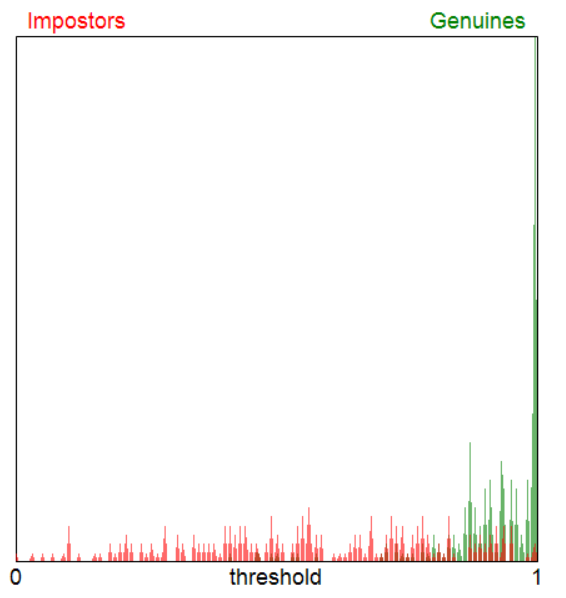
\includegraphics[width=.8\linewidth]{figures/score-distribution-red-eye-with-ycbcr.png}
    \caption{Distribuzione degli score per la metrica di rilevamento del difetto degli occhi rossi (versione yCbCr)}
    \label{fig:score_distribution_red_eye_with_ycbcr}
\end{figure}

\subsection{Valutazione metrica per il rilevamento dello sguardo frontale (metodo algoritmico)}
I risultati ottenuti tramite il metodo algoritmico rientrano nella media degli algoritmi pubblicati sulla piattaforma. \\[4pt]
\texttt{Equal Error Rate}: 17.1\%. \\
La distribuzione degli score è riportata nel grafico \Cref{fig:score_distribution_frontal_gaze_algo}.

\begin{figure}
    \centering
    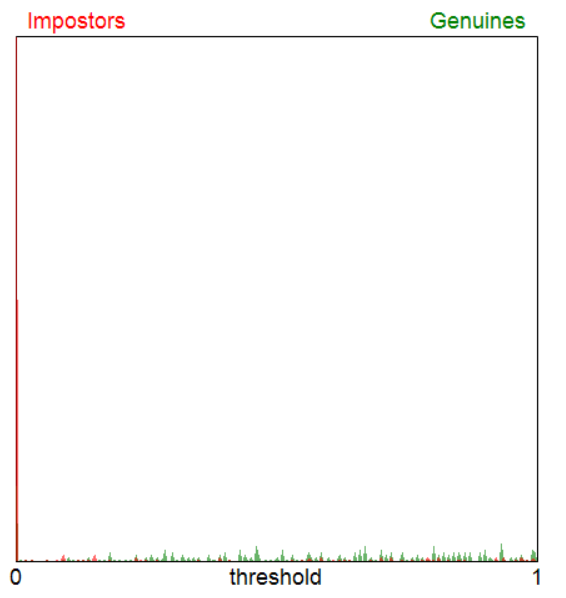
\includegraphics[width=.8\linewidth]{figures/score-distribution-frontal-gaze-algo.png}
    \caption{Distribuzione degli score per la metrica di rilevamento dello sguardo frontale (metodo algoritmico)}
    \label{fig:score_distribution_frontal_gaze_algo}
\end{figure}

\subsection{Valutazione metrica per il rilevamento dello sguardo frontale (metodo L2CS-Net)}
L'utilizzo della CNN L2CS-Net, in grado di predire l'angolatura dello sguardo, si è rivelato meno efficace del metodo algoritmico. \\[4pt]
\texttt{Equal Error Rate}: 12.9\%. \\
La distribuzione degli score è riportata nel grafico \Cref{fig:score_distribution_frontal_gaze_l2cs}.

\begin{figure}
    \centering
    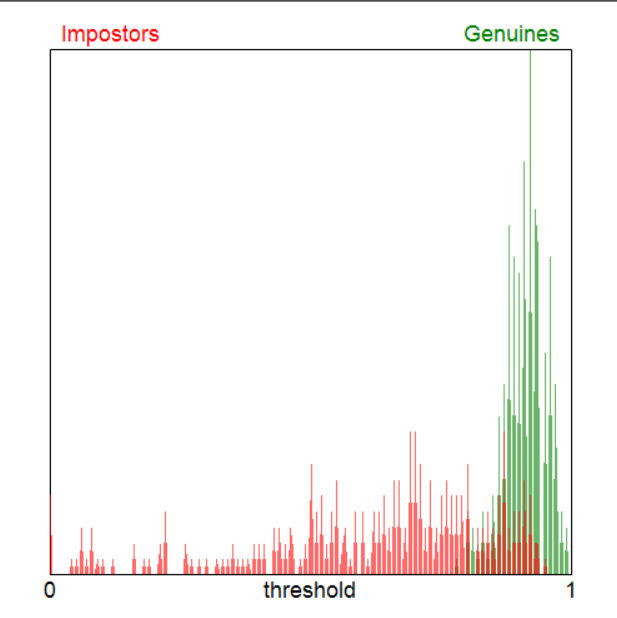
\includegraphics[width=.8\linewidth]{figures/score-distribution-frontal-gaze-l2cs.png}
    \caption{Distribuzione degli score per la metrica di rilevamento dello sguardo frontale (versione L2CS-Net)}
    \label{fig:score_distribution_frontal_gaze_l2cs}
\end{figure}

\section{Valutazione su dataset sintetici}

\subsection{Dataset utilizzati}
I dataset utilizzati per questa valutazione sono ONOT e TONO (già introdotti in precedenza). 
TONO fornisce immagini non conformi per i singoli difetti analizzati, mentre ONOT fornisce immagini conformi.

\subsection{Metriche valutate}
Nei dataset TONO e ONOT non è possibile valutare il difetto degli occhi rossi in quanto assente. 
La valutazione verrà effettuata sul solo difetto dello sguardo frontale.

\subsection{Procedimento di valutazione}
La valutazione delle metriche sui dataset ONOT e TONO è stata condotta secondo le seguenti fasi:
\begin{enumerate}
    \item \textbf{Filtraggio delle immagini in ONOT}: tramite i file TXT forniti con il dataset, sono state mantenute solo le immagini conformi allo standard ICAO.
    \item \textbf{Valutazione delle metriche in TONO}: ogni cartella di TONO e le rimanenti immagini di ONOT sono state valutate dal software OFIQ, generando file CSV contenenti, per ciascuna immagine, gli score assegnati alle metriche.
    \item \textbf{Analisi dei risultati}: le valutazioni delle immagini di TONO sono state confrontate con quelle di ONOT. Per ciascuna sottocartella di TONO, i risultati nella metrica relativa al difetto rappresentato sono stati messi in relazione con i corrispondenti risultati di ONOT.
    \item \textbf{Visualizzazione dei risultati}: per ogni metrica valutata, i risultati sono stati rappresentati con:
    \begin{itemize}
        \item \texttt{BoxPlot}: un confronto diretto tra distribuzioni di TONO e ONOT;
        \item \texttt{Distribuzione degli score}: un istogramma che confronta la distribuzione degli score (rosso = TONO, verde = ONOT);
        \item \texttt{Equal Error Rate}: misura dell'equilibrio tra falsi positivi e falsi negativi.
    \end{itemize}
\end{enumerate}

\subsection{Valutazione metrica per il rilevamento dello sguardo frontale (metodo algoritmico)}
\label{chap:evalutazione_frontal_gaze_algo}
Il dataset TONO contiene due cartelle con immagini relative al difetto dello sguardo frontale:
\begin{itemize}
    \item \textit{la\_1}: immagini di volti con lo sguardo rivolto verso destra;
    \item \textit{la\_2}: immagini di volti con lo sguardo rivolto verso sinistra.
\end{itemize}

\noindent Risultati per la cartella \textit{la\_1}: \\
\texttt{Equal Error Rate}: 15.8\%. \\
Distribuzione degli score: \Cref{fig:score_distribution_tono_onot_l1_frontal_gaze_algo}. \\
BoxPlot comparativo: \Cref{fig:box_plot_tono_onot_l1_frontal_gaze_algo}. \\

\noindent Risultati per la cartella \textit{la\_2}: \\
\texttt{Equal Error Rate}: 11.1\%. \\
Distribuzione degli score: \Cref{fig:score_distribution_tono_onot_l2_frontal_gaze_algo}. \\
BoxPlot comparativo: \Cref{fig:box_plot_tono_onot_l2_frontal_gaze_algo}. 


\begin{figure}[htbp]
    \centering
    \begin{subfigure}{0.49\textwidth}
        \centering
    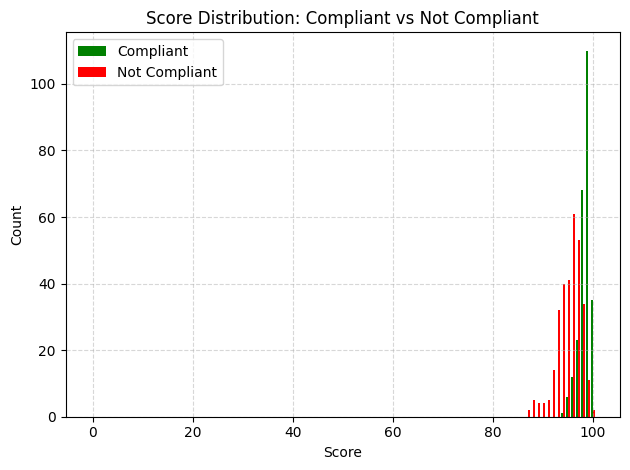
\includegraphics[width=.7\linewidth]{figures/score-distribution-tono-onot-l1-frontal-gaze-algo.png}
    \caption{Distribuzione degli score per il rilevamento dello sguardo frontale (metodo algoritmico), dataset TONO (cartella la\_1) e ONOT}
    \label{fig:score_distribution_tono_onot_l1_frontal_gaze_algo}
    \end{subfigure}
    \hfill
    \begin{subfigure}{0.49\textwidth}
        \centering
        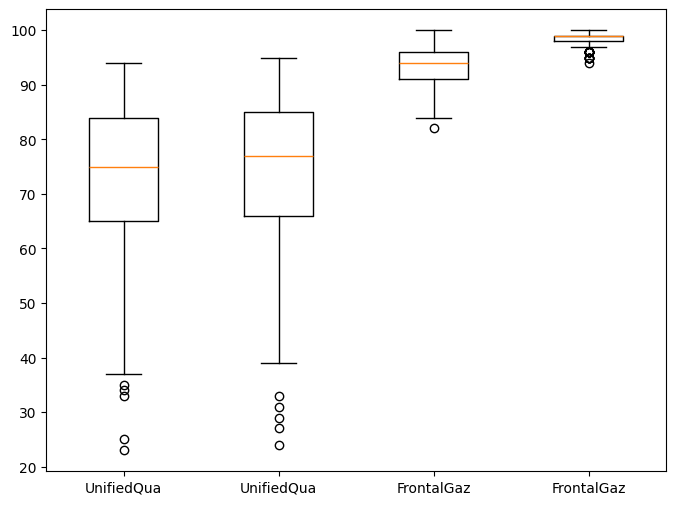
\includegraphics[width=.7\linewidth]{figures/box-plot-tono-onot-l1-frontal-gaze-algo.png}
        \caption{BoxPlot comparativo per il rilevamento dello sguardo frontale (metodo algoritmico), dataset TONO (cartella la\_1) e ONOT}
        \label{fig:box_plot_tono_onot_l1_frontal_gaze_algo}
    \end{subfigure}
    \begin{subfigure}{0.49\textwidth}
        \centering
        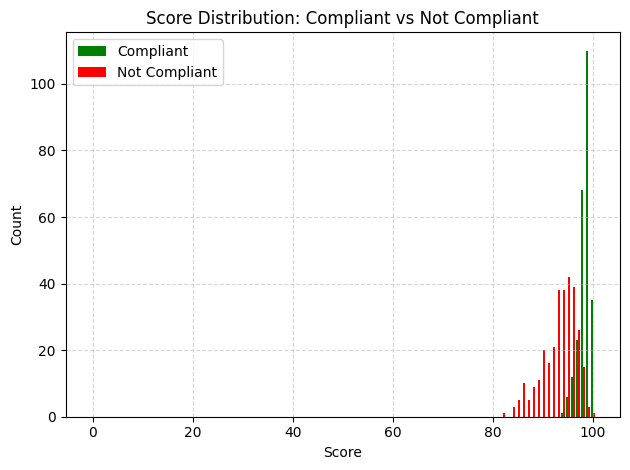
\includegraphics[width=.7\linewidth]{figures/score-distribution-tono-onot-l2-frontal-gaze-algo.png}
        \caption{Distribuzione degli score per il rilevamento dello sguardo frontale (metodo algoritmico), dataset TONO (cartella la\_2) e ONOT}
        \label{fig:score_distribution_tono_onot_l2_frontal_gaze_algo}
    \end{subfigure}
    \hfill
    \begin{subfigure}{0.49\textwidth}
        \centering
        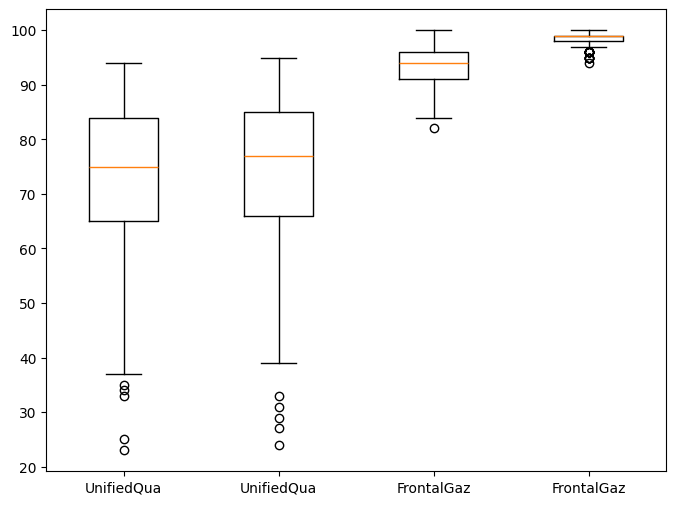
\includegraphics[width=.7\linewidth]{figures/box-plot-tono-onot-l2-frontal-gaze-algo.png}
        \caption{BoxPlot comparativo per il rilevamento dello sguardo frontale (metodo algoritmico), dataset TONO (cartella la\_2) e ONOT}
        \label{fig:box_plot_tono_onot_l2_frontal_gaze_algo}
    \end{subfigure}

    \caption{Grafici sulla valutazione della metrica del rilevamento dello sguardo frontale (metodo algoritmico)}
\end{figure}

\subsection{Valutazione metrica per il rilevamento dello sguardo frontale (metodo L2CS-Net)}
\label{chap:evaluatoin_l2csnet}
Come introdotto in precedenza, i risultati sono riportati separatamente per le cartelle \textit{la\_1} e \textit{la\_2}.

\noindent Risultati per la cartella \textit{la\_1}: \\
\texttt{Equal Error Rate}: 18.8\%. \\
Distribuzione degli score: \Cref{fig:score_distribution_tono_onot_l1_frontal_gaze_l2cs}. \\
BoxPlot comparativo: \Cref{fig:box_plot_tono_onot_l1_frontal_gaze_l2cs}. \\

\noindent Risultati per la cartella \textit{la\_2}: \\
\texttt{Equal Error Rate}: 18.6\%. \\
Distribuzione degli score: \Cref{fig:score_distribution_tono_onot_l2_frontal_gaze_l2cs}. \\
BoxPlot comparativo: \Cref{fig:box_plot_tono_onot_l2_frontal_gaze_l2cs}. 

\begin{figure}[htbp]
    \centering
    \begin{subfigure}{0.49\textwidth}
        \centering
        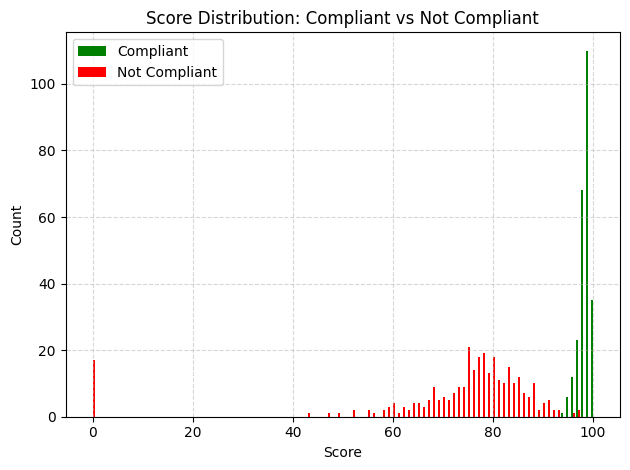
\includegraphics[width=.7\linewidth]{figures/score-distribution-tono-onot-l1-frontal-gaze-l2cs.png}
        \caption{Distribuzione degli score per il rilevamento dello sguardo frontale (metodo L2CS-Net), dataset TONO (cartella la\_1) e ONOT}
        \label{fig:score_distribution_tono_onot_l1_frontal_gaze_l2cs}
    \end{subfigure}
    \hfill
    \begin{subfigure}{0.49\textwidth}
        \centering
        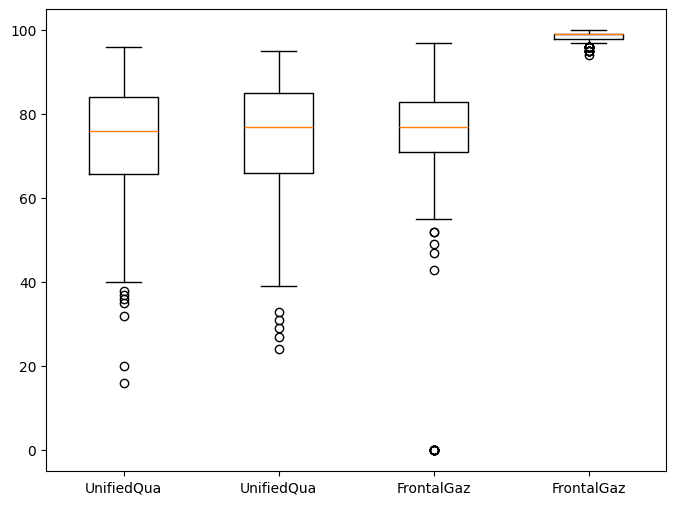
\includegraphics[width=.7\linewidth]{figures/box-plot-tono-onot-l1-frontal-gaze-l2cs.png}
        \caption{BoxPlot comparativo per il rilevamento dello sguardo frontale (metodo L2CS-Net), dataset TONO (cartella la\_1) e ONOT}
        \label{fig:box_plot_tono_onot_l1_frontal_gaze_l2cs}
    \end{subfigure}
    \begin{subfigure}{0.49\textwidth}
        \centering
        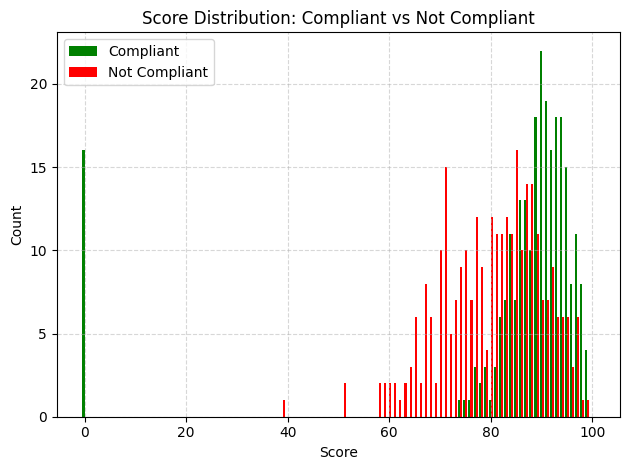
\includegraphics[width=.7\linewidth]{figures/score-distribution-tono-onot-l2-frontal-gaze-l2cs.png}
        \caption{Distribuzione degli score per il rilevamento dello sguardo frontale (metodo L2CS-Net), dataset TONO (cartella la\_2) e ONOT}
        \label{fig:score_distribution_tono_onot_l2_frontal_gaze_l2cs}
    \end{subfigure}
    \hfill
    \begin{subfigure}{0.49\textwidth}
        \centering
        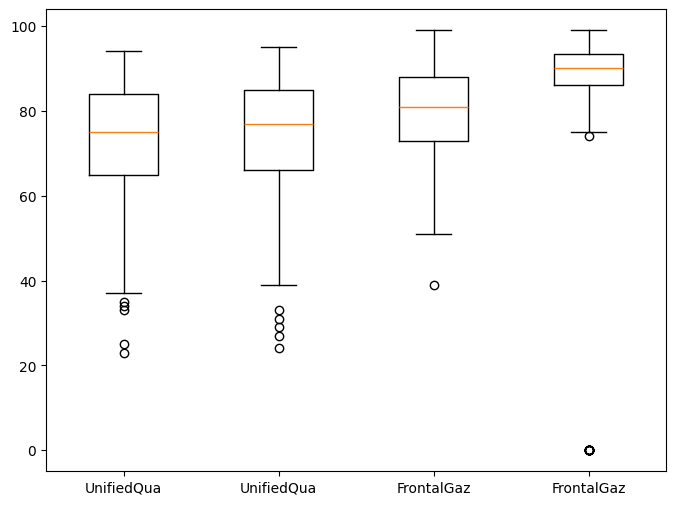
\includegraphics[width=.7\linewidth]{figures/box-plot-tono-onot-l2-frontal-gaze-l2cs.png}
        \caption{BoxPlot comparativo per il rilevamento dello sguardo frontale (metodo L2CS-Net), dataset TONO (cartella la\_2) e ONOT}
        \label{fig:box_plot_tono_onot_l2_frontal_gaze_l2cs}
    \end{subfigure}

    \caption{Grafici sulla valutazione della metrica del rilevamento dello sguardo frontale (metodo L2CS-Net)}
\end{figure}

\subsection{Valutazione dei modelli di machine learning sviluppati}
Di seguito sono riportati i valori di Equal Error Rate (EER) e la distribuzione degli score sui dataset TONO e ONOT per i modelli ottenuti tramite \textit{Fine-Tuning} di MobileNetV2 e per la CNN sviluppata da zero.

\paragraph{Versione 1, Fine-Tuning di MobileNetV2 sul dataset ``Gaze Direction Detection''} (Sezione~\ref{chap:mobilenetv2_ft_v1})
\begin{itemize}
    \item Dataset \texttt{la\_1} di TONO:  
    EER = 47.3\%, Score distribution: \Cref{fig:score_distribution_frontal_gaze_gdd_v1_la1}
    \item Dataset \texttt{la\_2} di TONO:  
    EER = 58.5\% , Score distribution: \Cref{fig:score_distribution_frontal_gaze_gdd_v1_la2}
\end{itemize}

\paragraph{Versione 2, Fine-Tuning di MobileNetV2 sul dataset ``Gaze Direction Detection''} (Sezione~\ref{chap:mobilenetv2_ft_v2})
\begin{itemize}
    \item Dataset \texttt{la\_1} di TONO:  
    EER = 46.9\%, Score distribution: \Cref{fig:score_distribution_frontal_gaze_gdd_v2_la1}
    \item Dataset \texttt{la\_2} di TONO:  
    EER = 58.0\%, Score distribution: \Cref{fig:score_distribution_frontal_gaze_gdd_v2_la2}
\end{itemize}

\paragraph{\texttt{gdd CNN}, Modello CNN sviluppato sul dataset ``Gaze Direction Detection''} (Sezione~\ref{chap:build_cnn_model})
\begin{itemize}
    \item Dataset \texttt{la\_1} di TONO:  
    EER = 38.4\%, Score distribution: \Cref{fig:score_distribution_frontal_gaze_gdd_v3_la1}
    \item Dataset \texttt{la\_2} di TONO:  
    EER = 21.8\%, Score distribution: \Cref{fig:score_distribution_frontal_gaze_gdd_v3_la2}
\end{itemize}

\medskip
Non sono state riportate le metriche su TONO e ONOT per i modelli basati sui landmark (Sezione~\ref{chap:landmark_based_model}), in quanto tali modelli sono stati addestrati direttamente su questi dataset. Per essi sono pertanto sufficienti le metriche calcolate sul test set.

\begin{figure}[htbp]
    \centering
    \begin{subfigure}{0.49\textwidth}
        \centering
        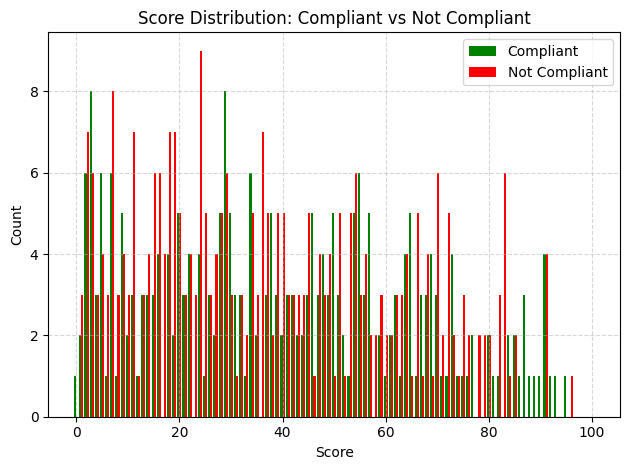
\includegraphics[width=.7\linewidth]{figures/score-distribution-frontal-gaze-gdd-v1-la1.png}
        \caption{Confronto con cartella \texttt{la\_1} di TONO}
        \label{fig:score_distribution_frontal_gaze_gdd_v1_la1}
    \end{subfigure}
    \hfill
    \begin{subfigure}{0.49\textwidth}
        \centering
        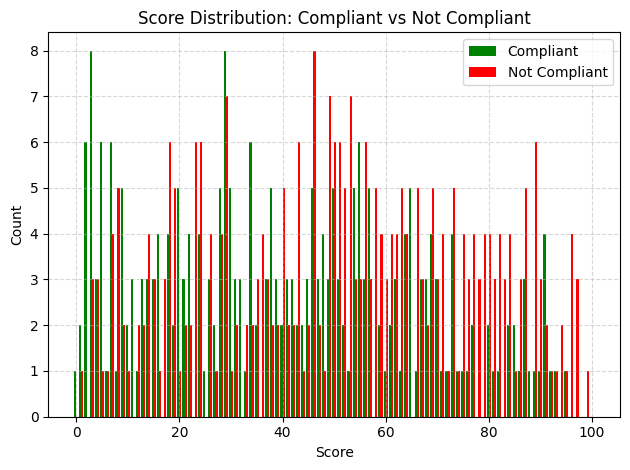
\includegraphics[width=.7\linewidth]{figures/score-distribution-frontal-gaze-gdd-v1-la2.png}
        \caption{Confronto con cartella \texttt{la\_2} di TONO}
        \label{fig:score_distribution_frontal_gaze_gdd_v1_la2}
    \end{subfigure}
    \caption{Distribuzione degli score per MobileNetV2 versione 1 su TONO e ONOT}
\end{figure}

\begin{figure}[htbp]
    \centering
    \begin{subfigure}{0.49\textwidth}
        \centering
        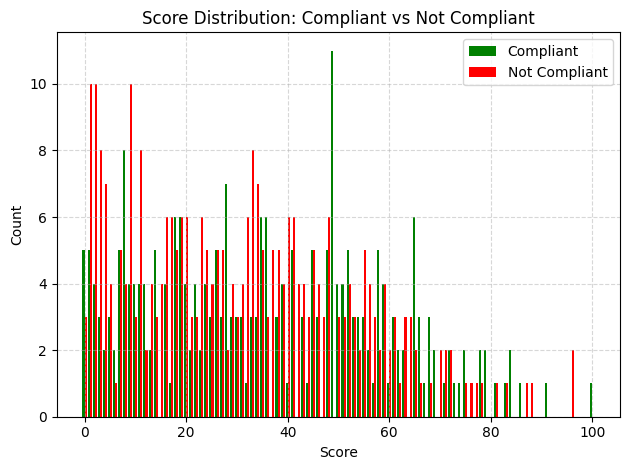
\includegraphics[width=.7\linewidth]{figures/score-distribution-frontal-gaze-gdd-v2-la1.png}
        \caption{Confronto con cartella \texttt{la\_1} di TONO}
        \label{fig:score_distribution_frontal_gaze_gdd_v2_la1}
    \end{subfigure}
    \hfill
    \begin{subfigure}{0.49\textwidth}
        \centering
        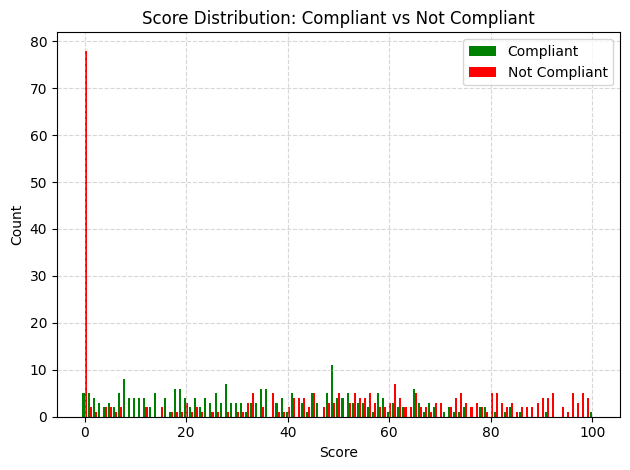
\includegraphics[width=.7\linewidth]{figures/score-distribution-frontal-gaze-gdd-v2-la2.png}
        \caption{Confronto con cartella \texttt{la\_2} di TONO}
        \label{fig:score_distribution_frontal_gaze_gdd_v2_la2}
    \end{subfigure}
    \caption{Distribuzione degli score per MobileNetV2 versione 2 su TONO e ONOT}
\end{figure}

\begin{figure}[htbp]
    \centering
    \begin{subfigure}{0.49\textwidth}
        \centering
        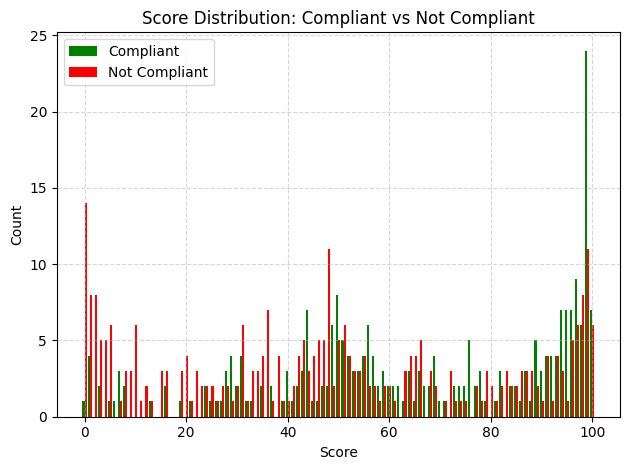
\includegraphics[width=.7\linewidth]{figures/score-distribution-frontal-gaze-gdd-v3-la1.png}
        \caption{Confronto con cartella \texttt{la\_1} di TONO}
        \label{fig:score_distribution_frontal_gaze_gdd_v3_la1}
    \end{subfigure}
    \hfill
    \begin{subfigure}{0.49\textwidth}
        \centering
        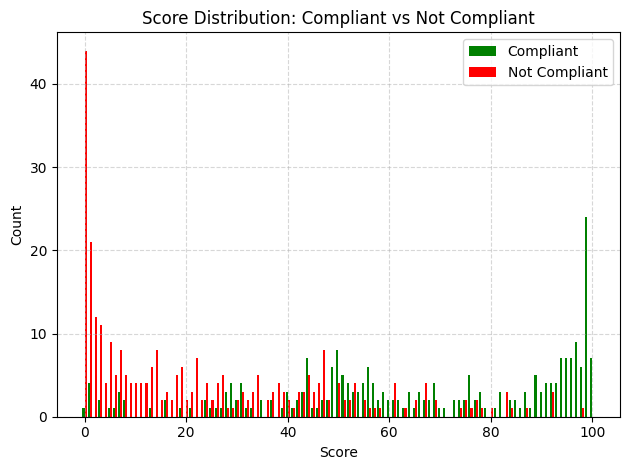
\includegraphics[width=.7\linewidth]{figures/score-distribution-frontal-gaze-gdd-v3-la2.png}
        \caption{Confronto con cartella \texttt{la\_2} di TONO}
        \label{fig:score_distribution_frontal_gaze_gdd_v3_la2}
    \end{subfigure}
    \caption{Distribuzione degli score per il modello \texttt{gdd CNN} su TONO e ONOT}
\end{figure}


\chapter{Analisi dei risultati}
\section{Rilevamento del difetto degli occhi rossi}
Nella metrica del rilevamento degli occhi rossi si è riscontrato un miglioramento delle performance nella versione che prevede l'utilizzo dello spazio colore YCBCR rispetto a quella con l'utilizzo dello spazio colore HSV, questo è dato dal fatto che il canale CR assume valori molto alti in presenza del colore rosso favorendone l'isolamento, inoltre l'informazione di luminanza è separata rispetto agli altri componenti rendendo il filtro più robusto a variazioni di luce/ombra. Si è inoltre analizzato che la non esclusione dei pixel della pupilla dal calcolo dei pixel totali dell'iride ha portato un ulteriore miglioramento delle performance, questo dovuto probabilmente dal fatto che il landmark non fosse correttamente centrato nella pupilla in alcuni casi portando ad escludere pixel utili alla conta dei pixel rossi totali. Un fattore che può aver inciso sull'equal error rate al 14\% può essere la sottomissione all'algoritmo di immagini riportanti difetti diversi da quello degli occhi rossi in immagini classficate con assenza di occhi rossi, come dimostrato dalle immagini \Cref{fig:red_eye_false_negative_images} che riportano score al 51 e 66 per colpa dell'errata saturazione dell'immagine, difetto riscontrabile da altre metiche implementate nel software OFIQ.
\begin{figure}[htbp]
    \centering
    \begin{subfigure}{0.49\textwidth}
        \centering
        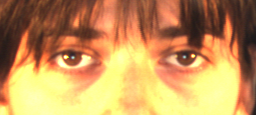
\includegraphics[width=.7\linewidth]{figures/red_eye_false_negative_image_1.png}
        \caption{Score: 51}
    \end{subfigure}
    \hfill
    \begin{subfigure}{0.49\textwidth}
        \centering
        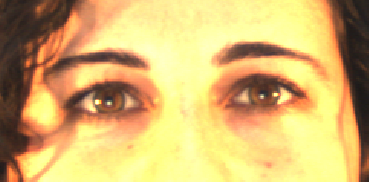
\includegraphics[width=.7\linewidth]{figures/red_eye_false_negative_image_2.png}
        \caption{Score: 66}
    \end{subfigure}
    \label{fig:red_eye_false_negative_images}
    \caption{Esempi di immagini false positivi alla metrica del rilevamento degli occhi rossi dal dataset Biolab}
\end{figure}

\section{Rilevamento del difetto dello sguardo frontale}
\subsection{Versione algoritmica}
Nelle valutazioni di questo metodo si può notare che le prestazioni migliori sono raggiunte su immagini generate artificialmente presentanti nessun altro difetto specifico, i casi di TONO e ONOT, e prestazioni inferiori sono invece riscontrate su immagini reali con eventuali altri difetti, come nel caso di FVC-Ongoing. Le debolezze di questo metodo includono immagini di volti nei quali i rapporti tra le distanze di punti specifi dell'occhio non sempre sono proporzionate (es. immagine classificata falsa negativi \Cref{fig:frontal_gaze_algo_weakness_3}, immagine classificata falsa negativa \Cref{fig:frontal_gaze_algo_weakness_1}, immagine classificata falsa positiva \Cref{fig:frontal_gaze_algo_weakness_4}), la dipendenza dell'algoritmo rispetto all'errore del modello che trova i landmark il quale in casi in cui sono presenti riflessi vicino o sopra gli occhi tende a trovare landmark distanti di qualche pixel rispetto a dove dovrebbero essere portando ad eventuali score minori e le immagini le quali riportano altri difetti quali una posa non frontale del viso (es. falso negativo \Cref{fig:frontal_gaze_algo_weakness_2}).

\begin{figure}[htbp]
    \centering
    \begin{subfigure}{0.49\textwidth}
        \centering
        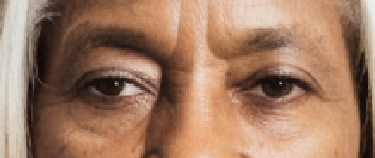
\includegraphics[width=.7\linewidth]{figures/frontal-gaze-algo-false-negative-94-1.png}
        \caption{Falso negativa, score: 94}
        \label{fig:frontal_gaze_algo_weakness_1}
    \end{subfigure}
    \hfill
    \begin{subfigure}{0.49\textwidth}
        \centering
        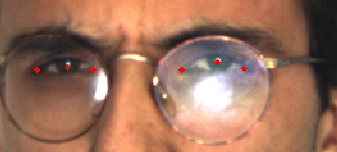
\includegraphics[width=.7\linewidth]{figures/frontal-gaze-algo-false-negative-80-2.png}
        \caption{Falso negativa, score: 80}
        \label{fig:frontal_gaze_algo_weakness_2}
    \end{subfigure}
    \begin{subfigure}{0.49\textwidth}
        \centering
        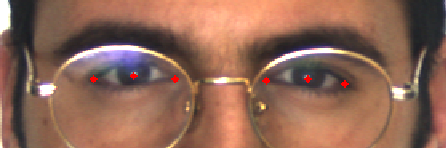
\includegraphics[width=.7\linewidth]{figures/frontal-gaze-algo-false-negative-0-3.png}
        \caption{Falso negativa, score: 0}
        \label{fig:frontal_gaze_algo_weakness_3}
    \end{subfigure}
    \begin{subfigure}{0.49\textwidth}
        \centering
        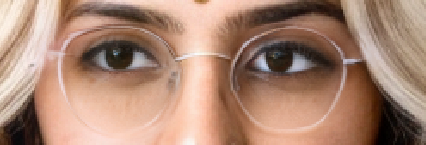
\includegraphics[width=.7\linewidth]{figures/frontal-gaze-algo-false-positive-98-1.png}
        \caption{Falso positiva, score: 98}
        \label{fig:frontal_gaze_algo_weakness_4}
    \end{subfigure}
    \label{fig:frontal_gaze_algo_weakness}
    \caption{Esempi di immagini false positivi e fale negativi nella metrica del rilevamento dello sguardo frontale con metodo algoritmico}
\end{figure}

\subsection{Versione con l'utilizzo del modello L2CS-Net}
Il metodo utilizzante il modello L2CS-Net è quello che meglio performa sulla piattaforma FVC-Ongoing piazzandosi al secondo posto tra i migliori risultati pubblicati sulla piattaforma. Nonostante ciò gli score ottenuti tramite questa metodologia sono ancora migliorabili. Un possibile miglioramento è dato dalla pipeline di preprocessing per la quale il modello l2cs si aspetta in input l'immagine di un volto rilevato dal modello \textit{RetinaFace} disponibile all'interno della libreria python ``face\_detection'', mentre per poter valutare il modello in OFIQ è stato utilizzato un altro modello di face detecting già presente in formato onnx all'interno di OFIQ.
In particolare nell'immagine \Cref{fig:frontal_gaze_l2cs_false_negative} l2cs-net, analizzando l'angolo yaw, usando \textit{RetinaFace} viene calcolato \texttt{0.03} radianti, mentre usando il modello all'interno di OFIQ viene calcolato \texttt{0.27} radianti, nonostante ciò, questo è un caso isolato, in quanto generalmente la differenza di predizione degli angoli nella media delle immagini è raramente superiore a \texttt{0.03} radianti.
Come possibile visualizzare nelle immagini \Cref{fig:frontal_gaze_l2cs_weakness}, esistono comunque casi in cui, sia usando \textit{RetinaFace} che usando il face detector di ONOT, il modello da score leggermente migliori ad un'immagine che sta guardando lateralmente (\Cref{fig:frontal_gaze_l2cs_false_positive})rispetto ad una che non lo sta facendo (\Cref{fig:frontal_gaze_l2cs_false_negative}), è però da segnalare che la prima immagini sia generata tramite modello di intelligienza artificiale generativa, mentre la seconda è un'immagine reale, questo evidenzia la tendenza del meteodo di dare score migliori ad immagini generate da intelligienza artificiale generativa.

\begin{figure}[htbp]
    \begin{subfigure}{0.49\textwidth}
        \centering
        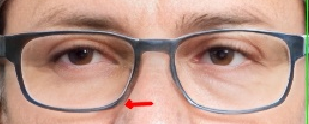
\includegraphics[width=.7\linewidth]{figures/frontal-gaze-l2cs-false-positive-97-1.png}
        \caption{Falso negativa, angolo pitch calcolato: 0.02}
        \label{fig:frontal_gaze_l2cs_false_positive}
    \end{subfigure}
    \hfill
    \centering
    \begin{subfigure}{0.49\textwidth}
        \centering
        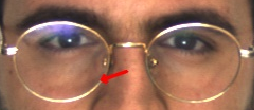
\includegraphics[width=.7\linewidth]{figures/frontal-gaze-l2cs-false-negative-65-1.png}
        \caption{Falso negativa, angolo pitch calcolato: 0.05}
        \label{fig:frontal_gaze_l2cs_false_negative}
    \end{subfigure}
    \label{fig:frontal_gaze_l2cs_weakness}
    \caption{Esempi di immagini false positivi e fale negativi nella metrica del rilevamento dello sguardo frontale con metodo L2CS-Net}
\end{figure}

\subsection{Versione con la costruzione e il fine tuning di modelli di machine learning}
I modelli addestrati nel Chapter~\ref{chap:frontal_gaze_with_ml} riportano nella maggior parte dei casi problemi di generalizzazione ottenendo score molto alti sul test-set, gdd CNN arriva all'85\% di accuratezza, non riescono poi ad ottenere score dello stesso livello una volta sottoposti ad altri dataset. In particolare i modelli ottenuti tramite Fine Tuning di MobileNetV2 sottoposti a Tono e Onot ottengono equal error rate che vanno dal 46 al 58 per cento rendendoli metodi inaffidabili. Inoltre anche sul sottodataset di Biolab contenente solamente immagini compliance e reali le performance non aumentano, riportando un'accuracy del \~40\%.
Ottiene performance migliori gdd CNN con Equal Error Rate su Tono e Onot che va dal 21 al 38 per cento circa, prestazioni comunque lontane da quelle ottenute con il metodo algoritmico (\ref{chap:evalutazione_frontal_gaze_algo}) e col metodo con L2CS-Net (\ref{chap:evaluatoin_l2csnet}). Sul sottodataset di Biolab ottiene un'accuracy del \~66\%. Nonostante le performance migliori dei fine tuning di MobileNetV2 il modello non può comunque essere ritenuto affidabile mostrando anch'esso difficolta nel generalizzazione una volta sottoposto a dataset differenti da quello di training.
I modelli basati sui landmark facciali anch'essi riportano score che li rendono attualmente non affidabili, ma è doveroso avere alcuni accorgimenti in merito, questa strategia deve essere considerata come uno spunto per l'approfondimento della tecnica. Il modello è stato addestrato con la totalità dei dati sintetici e con un dataset non bilanciato (2 immagini con sguardo non frontale ogni immagine con sguardo frontale) e di piccole dimensioni (un totale di \~1000 immagini divise in 80\% training set e 20\% test set). Questo test mette in mostra 2 cose principali, i modelli che utilizzano mediapipe come estrattore di landmark hanno anche score migliori e migliore capacità di generalizzazione, i modelli basati su XGBoost hanno equal error rate migliori di quelli basati sulla rete neurale keras e migliori capacità di generalizzazione.


\chapter{Conclusioni}

%----------------------------------------------------------------------------------------
% BIBLIOGRAPHY
%----------------------------------------------------------------------------------------

\backmatter

\nocite{*} % Remove this as soon as you have the first citation

\bibliographystyle{alpha}
\bibliography{bibliography}



\end{document}
